\documentclass[10pt,conference,letterpaper]{IEEEtran}
\IEEEoverridecommandlockouts
% The preceding line is only needed to identify funding in the first footnote. If that is unneeded, please comment it out.
\usepackage{cite}
\usepackage{amsmath,amssymb,amsfonts}
\usepackage{algorithmic}
\usepackage{graphicx}
\usepackage{textcomp}
\usepackage{xcolor}
\usepackage{booktabs}
\usepackage{bbding}
\usepackage{stfloats}
\usepackage{makecell}
\def\BibTeX{{\rm B\kern-.05em{\sc i\kern-.025em b}\kern-.08em
T\kern-.1667em\lower.7ex\hbox{E}\kern-.125emX}}
\begin{document}

    \title{Conference Paper Title*\\
    {\footnotesize \textsuperscript{*}Note: Sub-titles are not captured in Xplore and
    should not be used}
    \thanks{Identify applicable funding agency here. If none, delete this.}
    }

    \author{\IEEEauthorblockN{1\textsuperscript{st} Given Name Surname}
    \IEEEauthorblockA{\textit{dept. name of organization (of Aff.)} \\
    \textit{name of organization (of Aff.)}\\
    City, Country \\
    email address or ORCID}
%    \and
%    \IEEEauthorblockN{2\textsuperscript{nd} Given Name Surname}
%    \IEEEauthorblockA{\textit{dept. name of organization (of Aff.)} \\
%    \textit{name of organization (of Aff.)}\\
%    City, Country \\
%    email address or ORCID}
    }

    \maketitle

    \begin{abstract}
        This document is a model and instructions for \LaTeX.
    \end{abstract}

    \begin{IEEEkeywords}
        component, formatting, style, styling, insert
    \end{IEEEkeywords}


    \section{Introduction}

%In programming language theory(PLT), programming language design has always been an important topic. Because programming language design integrates various branches of PLT, it is the prerequisite for the final realization of programming language. By analyzing the design of modern programming languages(MPL), we can obtain the trend of programming language development, i.e., the programming language design can be fed back from the application point of view.
%
%By and large, the overall amount of literature on the analysis of
%programming language design is relatively small.
%M Coblenz argues that programming language design should be
%considered in terms of several theories related to programming
%languages and gives a way of evaluating programming language
%design\cite{coblenz2018interdisciplinary}.
%A Stefika gives some issues to consider in programming language
%design and argues that type systems are crucial for
%programming languages\cite{stefik2014programming}.
%However, the above results focus on a qualitative analysis of
%programming language design and lack some concrete examples.
%LA Meyerovich analyzes the usage of popular programming languages
%to give best practices in programming language design
%through statistics\cite{meyerovich2013empirical}.
%This analytical approach is somewhat lacking in theoretical and
%systematic aspects.
%F Morandat provides a systematic analysis of the R language,
%including performance, syntactic design, and application
%scenarios\cite{morandat2012evaluating}.
%The article adopts a better research approach and can be used to
%broaden the analysis perspective based on that article.
%Currently, there is a lack of a systematic, theoretical and
%practical, wide-ranging, application-oriented analysis of
%programming language design.
%
%By analyzing the design of MPL, this paper draws the influence of different programming language factors on the application. e.g., as programming languages evolve, why does the level of paradigm support in MPLs keep changing, what type systems are in MPLs, how MPLs keep programs efficient, and so on.

%%%%%%%%%%%%%%%%%%%%%%%%%
%In programming language theory (PLT), programming language
%design has always been an important topic.
%The design of a programming language would influence the way programmers think.
%Alan J. Perlis has said, “A language that doesn't affect the
%way you think about programming, is not worth knowing.”\cite{perlis1982special}
%
%
%However, the overall amount of literature on the analysis of
%programming language design is relatively small.
%M. Coblenz et.al argues that programming language design should be considered in terms
%of several related theories and proposes a way of evaluating programming
%language design\cite{coblenz2018interdisciplinary}.
%A. Stefika and S. Hanenberg give some issues to consider when designing
%a programming language and argues that type systems are crucial for
%programming languages\cite{stefik2014programming}.
%However, the above papers focus on qualitative analysis and lack
%some concrete examples.
%L. A. Meyerovich and A. S. Rabkin analyze the popularity of commonly
%used programming languages through statistics, which is relatively
%flawed in theoretical and systematic aspects\cite{meyerovich2013empirical}.
%F. Morandat et.al provides a systematic analysis of the R language,
%including performance, syntactic design, and application scenarios\cite{morandat2012evaluating}.
%The paper applies a relatively good method, but it analyzes only one language.
%
%
%In this paper, by analyzing the design of certain modern programming
%languages (MPLs) we chose, we conduct a systematic, theoretical and practical,
%and application-oriented analysis of the design of multiple programming languages.
%The trend of programming language development is obtained, and some design
%details are explained and discussed.
%Specifically, why the paradigm of MPLs keeps changing, what kind of
%type systems MPLs use, and how MPLs keep programs efficient.
%
%The paper is organized as following.
%Section 2 describes the features of MPLs and the criteria
%to evaluate the design of programming languages.
%Section 3 presents the analysis of paradigms of multiple MPLs we select in detail.
%Section 4 shows the results of type systems of the selected MPLs.
%Section 5 evaluate the performance of the selected MPLs.
%In Section 6, we give the conclusion.
%%%%%%%%%%%%%%%%%%%%%%%%%

In programming language theory (PLT), programming language
design has always been an important topic.
The design of a programming language would influence the way programmers think.
Alan J. Perlis has said, “A language that doesn’t affect the
way you think about programming, is not worth knowing.”\cite{perlis1982special}

However, the overall amount of literature on the analysis of
programming language design is relatively small.
M. Coblenz et.al argues that programming language design should be considered in terms
of several related theories and proposes a way of evaluating programming
language design\cite{coblenz2018interdisciplinary}.
A. Stefika and S. Hanenberg give some issues to consider when designing
a programming language and points out that type systems are crucial for
programming languages\cite{stefik2014programming}.
However, the above papers focus on qualitative analysis and lack
some concrete examples.
L. A. Meyerovich and A. S. Rabkin analyze the popularity of commonly
used programming languages through statistical counting,
which is relatively flawed in theoretical and systematic aspects\cite{meyerovich2013empirical}.
F. Morandat et.al provides a systematic analysis of the R language,
including performance, syntactic design, and application scenarios\cite{morandat2012evaluating}.
The paper applies a relatively good method, but it analyzes only one language.

%In this paper, we conduct a systematic, theoretical and practical,
%and application-oriented analysis of the design of multiple programming
%languages (MPLs).
%By analyzing the design of certain MPLs we chose, the trend of programming
%language development is obtained,
%and some design details are explained and discussed.
%Specifically, why the paradigm of MPLs keeps changing,
%what kind of type systems MPLs use, and how MPLs keep programs efficient.
In this paper, we conduct a systematic analysis of the design of
multiple modern programming languages (MPLs).
Our contribution is that, by analyzing programming paradigms, type systems, and performance of these languages' design,
we obtain their development trend to enable users to select suitable languages according to the application scene.


%The paper is organized as follows.
%Section 2 describes the features of MPLs and the criteria to evaluate the design of programming languages.
%Section 3 presents the analysis of paradigms of multiple MPLs we select in detail.
%Section 4 shows the results of type systems of the selected MPLs.
%Section 5 evaluates the performance of the selected MPLs.
%In Section 6, we give the conclusion.


    \section{Selecting several modern programming languages}

%We give the definition for MPL, accordingly choose nine MPLs,
%and explain the aspects of their designs to be analyzed.


%There is no uniform definition for MPL\@.
%Many researchers define it in different ways, such as finding
%connections between software engineering\cite{ModernProgrammingLanguagesSoftwareEnginerring}
%and the development of MPLs or elaborating
%around abstractions\cite{ModernProgrammingLanguagesAbstraction}.
%The above are correct in their respective fields,
%and here the definition is abstracted and extended to
%adapt to more domains.
%By studying the intersection of different definitions,
%a more general definition of MPLs derives.
%It is an obvious fact, that as the practice of
%programming languages continues to deepen, so does
%the definition of MPL. This is because PLT is a field
%where practice and theory go hand in hand.
%Although its definition is constantly changing, some
%core elements remain the same.
%Here are a few features of MPLs.

%\subsection{The features of modern programming language}

Researchers define MPL in different ways.
For example, some scholars define it from the perspective of software
engineering – as it develops, programming languages evolve into MPLs\cite{ModernProgrammingLanguagesSoftwareEnginerring}.
While others consider the key feature of MPL its abstraction\cite{ModernProgrammingLanguagesAbstraction}.
%In fact, as the practical technology of programming languages progresses,
%the definition of MPL will keep altering, because it is a combination
%of both theory and practice.
%However,although its definition keeps altering,
%some core contents remain unchanged.
%After studying multiple definitions given in the literature, we present a
%more general description for MPL, which has the following features:

%\begin{enumerate}
%    \item Substance over form. It should provide descriptive grammatical structures, rather than hand-in-hand telling the machine what to do. This item emphasizes the abstraction of machine functions.
%    \item Semantic consistency. For similar grammatical structures, there should be similar grammatical functions.
%    \item Syntax bootstrapping. For non-core grammatical features, based on following semantic consistency, they should be composed of core grammatical features.
%    \item Paradigm convergence. Multiple programming paradigms should be provided without forcing users to use a particular programming paradigm.
%\end{enumerate}

%\begin{enumerate}
%    \item Substance over form. MPLs should emphasize what is important to the users and restrain what is not.
%    \item Semantic consistency. For similar grammatical structures, there should be similar semantics.
%    \item Syntax bootstrapping. For non-core grammars, following semantic consistency, they should be composed of core grammars.
%    \item Paradigm convergence. Multiple programming paradigms should be provided without forcing users to use a particular one.
%\end{enumerate}

%\begin{table*}[hb]
%    \caption{Features that a well-designed programming language should have}
%    \label{tab:evaluate}
%    \begin{center}
%        \begin{tabular}{ccc}
%            \toprule
%            Evaluation Item & Meaning & Related Content \\
%            \midrule
%            Expressiveness &
%            \makecell[l]{
%                For abstract and complex business logic, programming \\
%                languages can provide a concise way to describe it.
%            }
%            & Programming Paradigm, Type System \\
%            \midrule
%            Maintainability &
%            \makecell[l]{
%                After completing the business logic according to \\
%                standard coding specifications, it is also easy to add new \\ features or
%                fix bugs subsequently.
%            }
%            & Programming Paradigm, Type System \\
%            \midrule
%            Reliability &
%            \makecell[l]{
%                Non-crash under extreme conditions after completing \\
%                business logic according to standard coding specifications.
%            }
%            & Programming Paradigm, Type System \\
%            \midrule
%            Performance &
%            \makecell[l]{
%                Deploying a software system written in this programming \\
%                language takes up fewer hardware resources when running \\ on the target
%                machine.
%            }
%            & Time Overhead, Memory Overhead \\
%            \bottomrule
%        \end{tabular}
%    \end{center}
%\end{table*}

%\subsection{Selecting modern programming languages to be analyzed}

%We select the MPLs to be analyzed based on the following considerations.
%We first select the current most popular programming languages.
%Next, there are many classification standards for programming languages.
%For each standard, the selected programming languages should cover most of the categories.
%Finally, we should focus on the new programming languages.
%These programming languages have absorbed the advantages of past languages and
%alleviated their inherent shortcomings.

According to the data of the IEEE spectrum,the top five popular programming
languages in 2021 are Python, Java, C, C ++, and JavaScript\cite{IEEETopProgrammingLanguages}.
Among them, C cannot be considered an MPL, due to its underlying syntax design.
We thus select the other four popular programming languages as our research objects.
According to the degree of popularity, we select five new-born MPLs -
Go, Swift, Dart, Rust, and Kotlin (where Swift and Dart are equally popular).
Coincidentally, these languages were also released in this order.
%It should be noted that, even though nowadays they are not exactly in line with the
%features of MPL, they were the representative symbols of MPLs back when they
%were initially developed.

%For the selection of programming language, the first thing is to pay attention to the most popular trend at the moment, so the selected programming language must cover the most commonly used. Secondly, there are many classification standards for programming languages. For each division standard, the selected programming language should cover most of the options. Then, it should focus on highlighting the new programming language with excellent design in recent years. These programming languages have absorbed the advantages of past programming languages and improved their inherent shortcomings. From these selected MPLs, we can see the development trend of application-oriented programming languages over the years.


%In addition, they all have similar type systems and support AOT compilation,
%and although not all of them use garbage collection memory management,
%they all move away from manual memory management.
%These are all common features of MPLs in today’s application environment.


%The timeline of the birth of the nine selected MPLs is shown in Figure~\ref{fig:timeline}.
%
%\begin{figure}[htbp]
%    \centerline{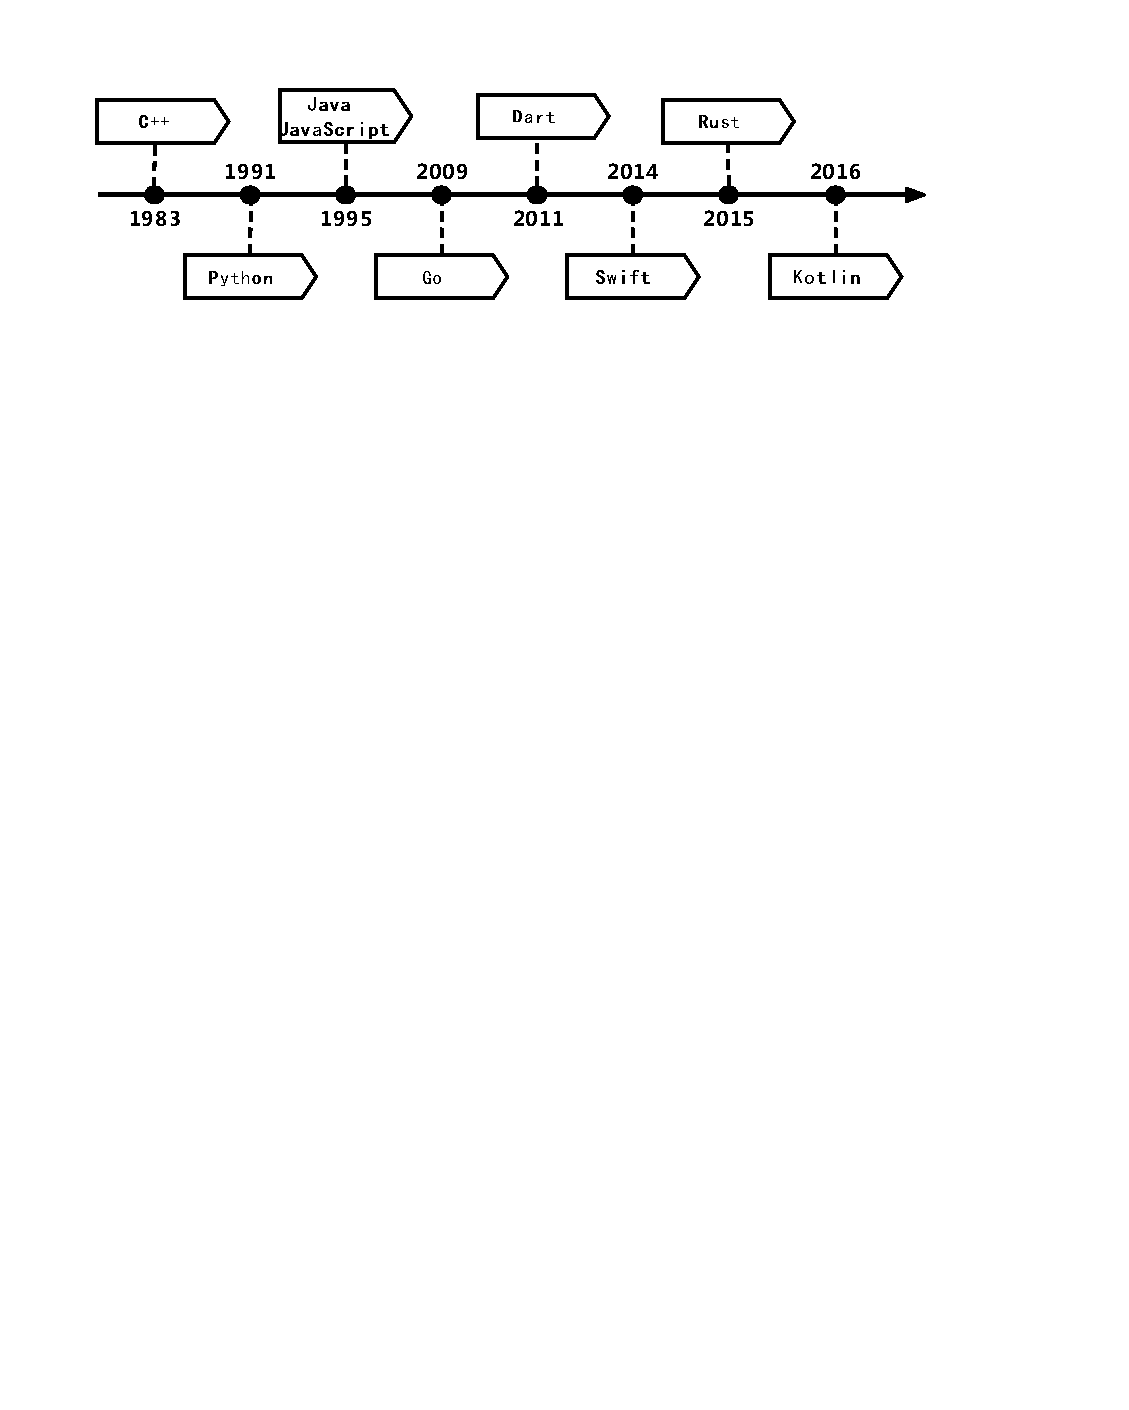
\includegraphics[scale=0.6]{figures/timeline}}
%    \caption{Timeline of several MPLs}
%    \label{fig:timeline}
%\end{figure}

%According to the data of the IEEE spectrum\cite{IEEETopProgrammingLanguages},
%the top five most popular programming languages in 2021 are Python, Java, C, C ++, and JavaScript. An exception case is C, which provides low-level access to computer systems. To be precise, the syntax design of the C language does not conform to any of the features of MPL. And for the four remaining popular programming languages mentioned above, they are still helpful even though they are not exactly in line with the features of MPL. In the era when these languages were first created, they emerged as representatives of MPLs. Therefore these four past programming languages are compared with the emerging MPLs.


%Based on the above-mentioned MPL features,
%several programming languages were selected and arranged
%in order of popularity\cite{IEEETopProgrammingLanguages},
%resulting in Go, Swift, Dart, Rust and Kotlin (where Swift and Dart are equally popular).
%%Coincidentally, these languages are also released in this order sequentially, see Figure\ref{fig:timeline}.
%%In addition, all of these languages have similar type systems and all support AOT compilation, and although not all use garbage collection memory management, they all move away from manual memory management.
%%These are all common features of MPLs in today's application environment, as we can see from Table\ref{tab:selected-languages}.

%\subsection{Criteria to evaluate the design of programming languages}


%We think there are two main aspects that determine whether a language is useful or not.
%One aspect is its syntactic design.
%For complex business logic, programming languages are required to provide
%strong expressiveness, i.e., isolate underlying implementations
%that are not related to the business logic to accommodate rapid changes.
%Programming languages are also needed to provide solutions for
%checking the correctness and reliability of programs.
%Another aspect is performance, where programming languages are
%always expected to have a low memory overhead and time overhead,
%relying heavily on compile-time (native languages) and run-time
%(virtual machine languages) optimizations.
%See Table\ref{tab:evaluate}.


We assess the designs of these MPLs from an application-oriented point of view.
In other words, we evaluate whether a language design is “practical”.
There are mainly two aspects that determine whether a language is practical or not.
One is its syntactic design.
To deal with complex business logic, programming languages are expected to be strong expressive,
which correlated with its paradigms.
%i.e., isolate underlying implementations that are not related to the business logic to
%accommodate rapid changes.
Programming languages also need to provide solutions for correctness checking,
which correlated with its type systems.
Ultimately, programming languages are always supposed to have a better performance,
which rely heavily on compile-time (native languages) and run-time (virtual machine languages) optimizations.
%Specifically, the evaluation criteria of this paper are presented in Table~\ref{tab:evaluate}.
%For expressiveness, maintainability, and reliability of a language, we analyze them
%by programming paradigm or type system;
%for Performance of a language, we analyze it by time overhead and memory overhead.
And the profile of the nine selected MPLs about their programming paradigm,
type system, compilation mode and memory model are shown in Table~\ref{tab:selected-languages}.

\begin{table*}[htbp]
    \caption{Several modern programming languages}
    \label{tab:selected-languages}
    \begin{center}
        \begin{tabular}{ccccccc}
            \toprule
            Language & Programming Paradigm & Type System & Compilation Mode & Memory Model &
            Release Date & Application Scenarios \\
            \midrule
            Python & Multi-paradigm & Dynamically, Strongly & JIT & GC & 1991 & Web,
            Enterprise, Embedded \\
            Java & Multi-paradigm & Statically, Strongly & AOT & GC & 1995 & Web,
            Mobile, Enterprise \\
            C++ & Multi-paradigm & Statically, Weakly & AOT & Manual & 1983 & Mobile,
            Enterprise, Embedded \\
            JavaScript & Multi-paradigm & Untyped & JIT & GC & 1995 &
            Web \\
            Go & Multi-paradigm & Statically, Strongly & AOT & GC & 2009 & Web,
            Enterprise \\
            Swift & Multi-paradigm & Statically, Strongly & AOT & ARC & 2014 &
            Mobile, Enterprise \\
            Dart & Multi-paradigm & Statically, Strongly & AOT\&JIT & GC & 2011 &
            Web, Mobile \\
            Rust & Multi-paradigm & Statically, Strongly & AOT & Ownership & 2015 &
            Web, Enterprise, Embedded \\
            Kotlin & Multi-paradigm & Statically, Strongly & AOT\&JIT & GC & 2016 &
            Web, Mobile \\
            \bottomrule
        \end{tabular}
    \end{center}
\end{table*}

%In practice, however, programming language design cannot be accurately quantified.
%The reason for this is twofold.
%The first is that certain criteria for evaluation are not quantitative.
%For expressiveness and reliability, both are abstract descriptions,
%and they have uncountable kinds of cases in practice.
%If one wants to analyze them quantitatively, then one must restrict the analysis to
%certain specific application scenarios.
%The second is that the evaluation criteria are not sufficient.
%Some evaluation criteria that are difficult to measure, such as response time in a
%real-time system, are dropped here for structural completeness.
%For programming languages with garbage collectors, the performance loss from garbage collection is not negligible. In particular, JVM-based programming languages have the problem of "Stop the World" when garbage collection is performed, which affects the performance of the programming language. However, this is not considered for the sake of simplicity.


%It should be emphasized that programming language design cannot be fully
%evaluated by quantitative analysis.
%For expressiveness and reliability, which are descriptions for abstract concepts,
%although quantitative analysis is possible, it is usually limited to a certain
%application environment, which does not have much significance.
%Some other performances are difficult to measure, such as response time in real-time systems.
%Additionally, for programming languages with garbage collectors, the performance
%loss from garbage collection is not negligible.
%In particular, JVM-based programming languages have the problem of "Stop the World"
%when garbage collection is performed\cite{gidra2013study},
%which affects the performance of the programming language.
%Such features are not considered in this paper.
    \section{How to evaluate the design of programming languages}

The evaluation criteria here are more application-oriented, to evaluate whether a programming language is "practical" or not. Rather than evaluating whether a programming language is "elegant" as in the features of MPL. In fact, most of the popular languages are not elegant. This is because the development of programming languages is not just a technical matter, but involves political, commercial, and other external factors. A typical example is the evolution of JavaScript. Today, the language standards for JavaScript in mainstream browsers are still not uniform. But this does not prevent JavaScript from being the most popular language for Web applications. But that doesn't stop JavaScript from being the most useful language for Web applications. There are two main aspects that determine whether a language is useful or not. One aspect is its syntactic design. For complex business logic, programming languages are required to provide strong expressiveness, i.e., isolate underlying implementations that are not related to the business logic to accommodate rapid changes. Programming languages are also needed to provide solutions for checking the correctness and reliability of programs. Another aspect is performance, where programming languages are always expected to have a low memory overhead and time overhead, relying heavily on compile-time (native languages) and run-time (virtual machine languages) optimizations.

\begin{table*}[ht]
    \caption{evaluate}
    \label{tab:evaluate}
    \begin{center}
        \begin{tabular}{ccc}
            \toprule
            Evaluation Item & Meaning & Related Content \\
            \midrule
            Expressiveness &
            \makecell[l]{
                For abstract and complex business logic, programming \\
                languages can provide a concise way to describe it.
            }
            & Programming Paradigm, Type System \\
            \midrule
            Maintainability &
            \makecell[l]{
                After completing the business logic according to \\
                standard coding specifications, it is also easy to add new \\ features or
                fix bugs subsequently.
            }
            & Programming Paradigm, Type System \\
            \midrule
            Reliability &
            \makecell[l]{
                Non-crash under extreme conditions after completing \\
                business logic according to standard coding specifications.
            }
            & Programming Paradigm, Type System \\
            \midrule
            Performance &
            \makecell[l]{
                Deploying a software system written in this programming \\
                language takes up fewer hardware resources when running \\ on the target
                machine.
            }
            & Time Overhead, Memory Overhead \\
            \bottomrule
        \end{tabular}
    \end{center}
\end{table*}

\textcolor{red}{!!!!!!!!!machine translation!!!!!!!!!}

In practice, however, programming language design cannot be accurately quantified. The reason for this is twofold. The first is that certain evaluation criteria are not quantitatively analyzed. For expressiveness and reliability, both are descriptions of abstract concepts, reflecting the fact that there are uncountable kinds of situations in practice that cannot all be taken into account. Although a quantitative analysis can be designed, it has to be done by limiting certain specific application scenarios. The second is that the criteria for evaluation are not sufficient. For the sake of structural completeness of the paper, some evaluation criteria that are difficult to measure, such as response time in real time systems, are dropped. For programming languages with garbage collection mechanisms, the performance loss from garbage collection is not negligible. In particular, JVM-based programming languages have the problem of "Stop the World" when garbage collection is performed, which can affect the performance of the programming language. However, this is not considered for the sake of simplicity.



    \section{Programming paradigm}

Programming paradigms are derived from the way people perceive the real world, and programming languages are tools for formally describing this way of perception. When people develop software, they model the real world in a computer, and the different programming paradigms lie in the different ways of modeling the real world. Modeling the world often requires solving two problems. The first is to find out what the basic units of the world are, called first-class citizens. These first-class citizens can be stored in variables, passed as function parameters and function return values, in short, the "data" to be manipulated in a program. The second is to find out the relationship between these basic units, called computation. Computation can be seen as the "manipulation" of data in a program. For example, object-oriented treats objects as first-class citizens, and computations between objects are called methods. Another example is functional style, where functions are considered first-class citizens and computations are lambda calculations, which are computations on the functions themselves. Interestingly, functions in functional style are both the basic unit and the form of computation.

The programming paradigm is the lowest level of design for programming languages. Theoretically, programming languages need to help people to do the modeling of the real world, and therefore need to consider what modeling infrastructure should be provided, i.e., the programming paradigm of the programming language. Practically speaking, the design of a programming language should first consider the first-class citizen as the basic unit of the programming language. There is a certain conflict between different programming paradigms, stemming from the conflict of first-class citizens. In particular, it is very difficult to add a new paradigm to a programming language that defines the paradigm. A typical example is Java. the functional features added by Java8 do not fundamentally change the programming paradigm of Java, but are at best syntactic sugar. The lack of the original programming paradigm design makes it difficult for Java to be fully compatible with functional features, and thus the functional style in Java is crippled and inelegant. Therefore, for programming languages, especially for modern programming languages with multiple paradigms, the programming paradigm, and thus the first-class citizens, should be determined first.

Functional programming (FP) and object-oriented programming (OOP) are the two most common, and at the same time the most important, paradigms in modern programming languages. Therefore, these two paradigms are chosen for analysis when discussing programming paradigms below.

\subsection{Languages, paradigms, and concepts}

\begin{figure}[htbp]
    \centerline{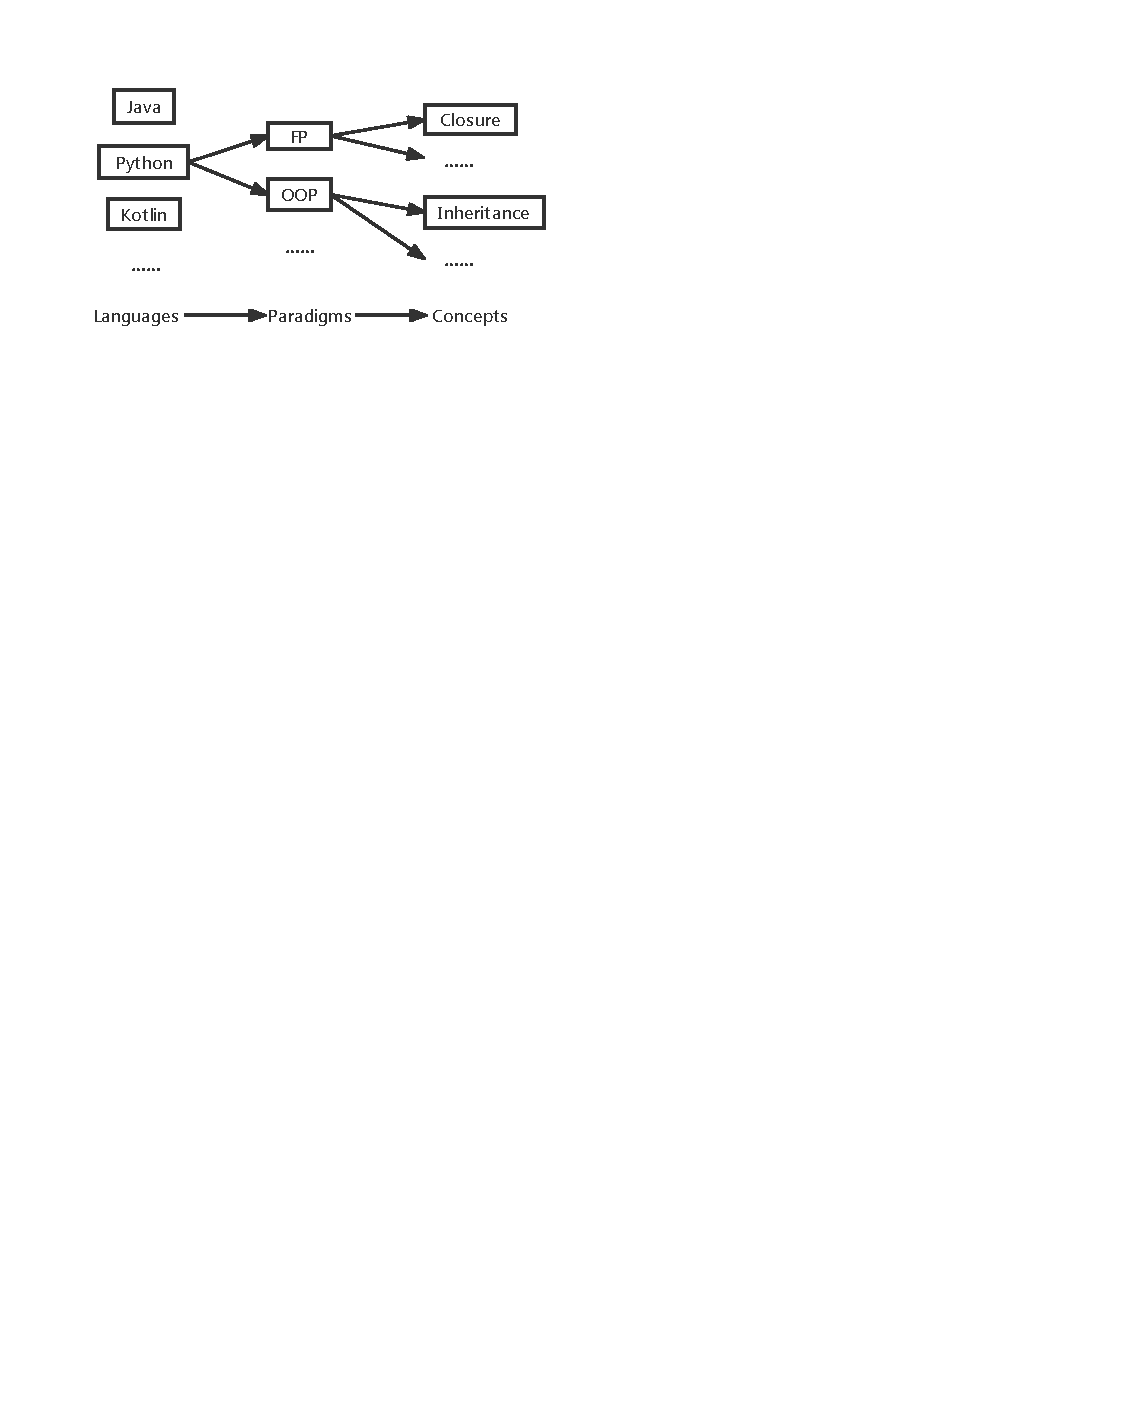
\includegraphics[scale=0.8]{figures/concept}}
    \caption{concept}
    \label{fig:concept}
\end{figure}

The diagram shows the relationship between languages, paradigms, and concepts. Each paradigm contains a core set of concepts, and at the same time, each language implements multiple paradigms. Functional and object-oriented are the programming paradigms typically found in modern programming languages. The degree of support for them varies across programming languages, and the table shows the degree of support for functional and object-oriented concepts in each language.

For the concepts that make up the programming paradigm, a more practically oriented organization is chosen here. It will favor the selection of concepts defined in specific programming languages rather than those defined in programming paradigm theory. For example, for the functional concept of nested and anonymous functions, they are implemented in many programming languages as lambda expressions. Another example is for the object-oriented concept of composition, which is supported by most of the currently popular programming languages. In fact, for programming language design itself, composition is simply a way of arranging data, it does not belong to any paradigm. Even languages like the more ancient one, C, provide structure combinations and function combinations. Therefore, it is not included in the analysis.

\begin{table*}[ht]
    \caption{concept}
    \label{tab:concept}
    \begin{center}
        \begin{tabular}{cll}
            \toprule
            Paradigm & Concept & Meaning \\
            \midrule
            FP & Higher-order functions & Take functions as variables, which can
            pass as parameters or return values. \\
            FP & Lambda expression & A short block of code which takes in parameters
            and returns a value. \\
            FP & Partial application & Given a function with certain parameters,
            producing another function (with fewer parameters). \\
            FP & Closures & A record stores a function together with an
            environment\cite{sussman1998scheme}. \\
            FP & Type inference & The automatic detection of the type of an
            expression at compile time. \\
            FP & Pattern matching & Dispatch branch by matching the pattern of a
            given sequence of tokens. \\
            FP & Statement as expression & Take all statements as expressions, which
            creates a definite value. \\
            OOP & Encapsulation & Hide the properties and implementation details of
            the object, and only expose the interface to the outside. \\
            OOP & Inheritance & Create classes that are built upon existing
            classes\cite{johnson1988designing}. A way of
            code reuse. \\
            OOP & Composition & Combine entities into more complex ones. A way of
            code reuse. \\
            OOP & Delegation & One entity passing something to another
            entity\cite{wilkinson2009grid}. A way of code
            reuse. \\
            OOP & Traits & A set of method conventions. Broadly including trait,
            interface, protocol and mixin. \\
            OOP & Polymorphism & Use of a single symbol to represent multiple
            different
            types\cite{cardelli1985understanding}. \\
            OOP & Everything is object & All the basic elements of a programming
            language are represented in the form of objects. \\
            \bottomrule
        \end{tabular}
    \end{center}
\end{table*}

\subsection{Functional programming}

The most important feature of functional programming is its high degree of abstraction. This is mainly because functional programming has its roots in the lambda calculus, so it has some of the characteristics of abstract algebra. In the practice of functional languages, the main idea is the combination and nesting of higher-order functions, so the core of its design is to sort out the rules of nesting and combination of higher-order functions. Therefore, the basic design method can be described as follows: through the standardization of the function transfer model and the combinability of higher-order functions, the description of the mapping of data from the source to the result is completed through a series of rule designs. The mapping here is accomplished by the formal combination of multiple higher-order functions. The description is like a mathematical formula that maps the input data into the result through layers of iterations. For the iterative process of data in a broad sense, this includes not only the iteration of the data itself, but also the iteration of the rules. This is due to the fact that in functional languages, data and rules are semantically unified in functions.

This leads to the characteristics of functional programming.

\begin{enumerate}
    \item High expressiveness. Functional programming is a data-driven expression with a high degree of abstraction, so that business logic can be accomplished with very little code within the scope of its expression.
    \item High maintainability within certain limits. First, functional programming is declarative expression and easy to understand. Second, higher-order functions are less granular and more composable. But its high maintainability is subject to certain conditions. First, the business logic is complex and not logically self-consistent in every aspect, so finding a complete set of rules to map is difficult. Second, both the rules of mapping are found in a narrow domain, but once it needs to be expanded to a new domain, the original rules will fail.
    \item High reliability. Since functional languages are based on lambda calculus, formal verification of functional code is relatively easy. Thus correctness and reliability can be guaranteed.
    \item Poor performance on Turing machines. In functional languages, there are more intermediate layers between the syntax rules and the Turing machine, as well as its syntax rules and inert evaluation, which makes optimization more difficult.
\end{enumerate}

\begin{table*}[ht]
    \caption{fp}
    \label{tab:fp}
    \begin{center}
        \begin{tabular}{cccccccc}
            \toprule
            Language & Higher-order functions & Lambda expression & Partial
            application & Closures & Type inference & Pattern matching & Statements
            as expressions\\
            \midrule
            Python     & \Checkmark & \Checkmark & Python2.5   & \Checkmark & \Checkmark & Python3.10  & ×          \\
            Java       & Java8      & Java8      & Java8       & Java8      & Java10     & ×           & ×          \\
            C++        & C++11      & C++11      & C++11       & C++11      & C++11      & C++17       & ×          \\
            JavaScript & \Checkmark & \Checkmark & ECMAScript5 & \Checkmark & \Checkmark & ECMAScript6 & ×          \\
            Go         & \Checkmark & \Checkmark & \Checkmark  & \Checkmark & \Checkmark & ×           & ×          \\
            Swift      & \Checkmark & \Checkmark & \Checkmark  & \Checkmark & \Checkmark & \Checkmark  & ×          \\
            Dart       & \Checkmark & \Checkmark & \Checkmark  & \Checkmark & \Checkmark & ×           & ×          \\
            Rust       & \Checkmark & \Checkmark & \Checkmark  & \Checkmark & \Checkmark & \Checkmark  & \Checkmark \\
            Kotlin     & \Checkmark & \Checkmark & \Checkmark  & \Checkmark & \Checkmark & \Checkmark  & \Checkmark \\
            \bottomrule
        \end{tabular}
    \end{center}
\end{table*}

As programming language practice has deepened, programming languages have become more and more supportive of functional concepts. With for the programming languages released in the 1980s and 1990s, the support for functional style was not good when programming languages were first created. In particular, Java and C++, from their initial syntax, were not designed with functional programming in mind. This is better for JavaScript and Python, which inherently support functional style, but still lack some advanced functional concepts. For programming languages released around 2010, the basic concepts of functionalism are supported. Rust and Kotlin, in particular, additionally support the concept of "Statements as expressions", a milestone in the development of modern programming language paradigm convergence. The concept of "statements as expressions", which is more common in functional languages, enables semantic unification of expressions and statements, but is not implemented in most programming languages that integrate object-oriented and functional paradigms. As programming languages continue to evolve, Kotlin and Rust have implemented a fusion of functional and object-oriented paradigms that includes this concept, so Kotlin and Rust can be considered as functional paradigms with a higher level.

\subsection{Object oriented orogramming}

The most important feature of object orientation is the emphasis on reuse. Back in the 1960s, software maintenance became increasingly difficult due to the increasing complexity of software and hardware. Object-Orientation solves this problem by emphasizing reusability. In the practice of object-oriented languages, people mapped real problems into entities and their relationships, rather than caring about the process of dealing with the problem. After the birth of object-oriented languages, there was an urgent need for a modeling approach that mapped problems into entities and relationships, at which point UML was born. It is a standardized modeling language consisting of a set of icons that has greatly contributed to the development of object-oriented methodologies. This approach emphasizes the importance of modeling and design.


In the same way, the characteristics of object-oriented programming can be obtained.

\begin{enumerate}
    \item A certain expressiveness. While encapsulation increases the level of code abstraction, it essentially shifts and splits the business logic. In addition, the complex hierarchical structure of object-oriented reduces its expressiveness. Design patterns emerge to compensate for the shortcomings of object-oriented expression.
    \item High maintainability. First, the object itself is highly reusable and applicable to more areas. Second, polymorphism improves the ability to respond to change. Third, encapsulation facilitates the cost of understanding for maintainers.
    \item A certain degree of reliability. Object-oriented modeling relies on practical experience and lacks rigorous theoretical proof. The usual best practices for object-oriented modeling are limited to the realm of inductive methods.
    \item Better performance. Object-oriented can achieve near-native performance of Turing machines. Most of the performance overheads, such as dynamic binding, function call overheads, can be optimized by compilation means.
\end{enumerate}


And there is not much difference in the level of support for the core object-oriented concepts in popular languages. Because of their long history of development and no major theoretical or practical innovations in recent years, most programming languages have implemented the core object-oriented concepts relatively completely. In addition, more and more programming languages are implementing object-oriented features by supporting combinations and delegates, while mere inheritance has proven to be bad practice. As a result, the concepts of classes and inheritance have been abandoned in Go and Rust, and traditional object-orientation is implemented through trait. Compared to class-based object-orientation, trait-based object-orientation is more loosely coupled and more flexible to implement. However, most languages support both trait and class to enable different granularity of control.

To more accurately distinguish the strengths and weaknesses of each language's object-oriented programming paradigm, some less common concepts are introduced here. One example is "everything is object". According to the definition of object-oriented, it should have been the core concept in object-oriented. But in fact, early programming languages tended to have a lot of imperative features, and not all elements of a programming language were treated as objects. For example, there are still "primitive data types" in Java, which are not objects, so we cannot call methods of these types as if they were objects. There may be many performance positives of "primitive data types", but from a semantic consistency point of view, "primitive data types" have a negative effect. Therefore, languages with the concept of "everything is object" are considered to have better object-oriented features.

\begin{table*}[ht]
    \caption{oop}
    \label{tab:oop}
    \begin{center}
        \begin{tabular}{cccccc}
            \toprule
            Language & Inheritance & Delegation & Traits & Polymorphism &
            Everything is object \\
            \midrule
            Python     & \Checkmark & \Checkmark & ×          & \Checkmark & \Checkmark \\
            Java       & \Checkmark & ×          & \Checkmark & \Checkmark & ×          \\
            C++        & \Checkmark & ×          & \Checkmark & \Checkmark & ×          \\
            JavaScript & \Checkmark & \Checkmark & ×          & \Checkmark & \Checkmark \\
            Go         & ×          & ×          & \Checkmark & \Checkmark & ×          \\
            Swift      & \Checkmark & ×          & \Checkmark & \Checkmark & \Checkmark \\
            Dart       & \Checkmark & ×          & ×          & \Checkmark & \Checkmark \\
            Rust       & ×          & \Checkmark & \Checkmark & \Checkmark & \Checkmark \\
            Kotlin     & \Checkmark & \Checkmark & \Checkmark & \Checkmark & \Checkmark \\
            \bottomrule
        \end{tabular}
    \end{center}
\end{table*}

\subsection{Programming Paradigms and Applications}

\begin{figure}[htbp]
    \centerline{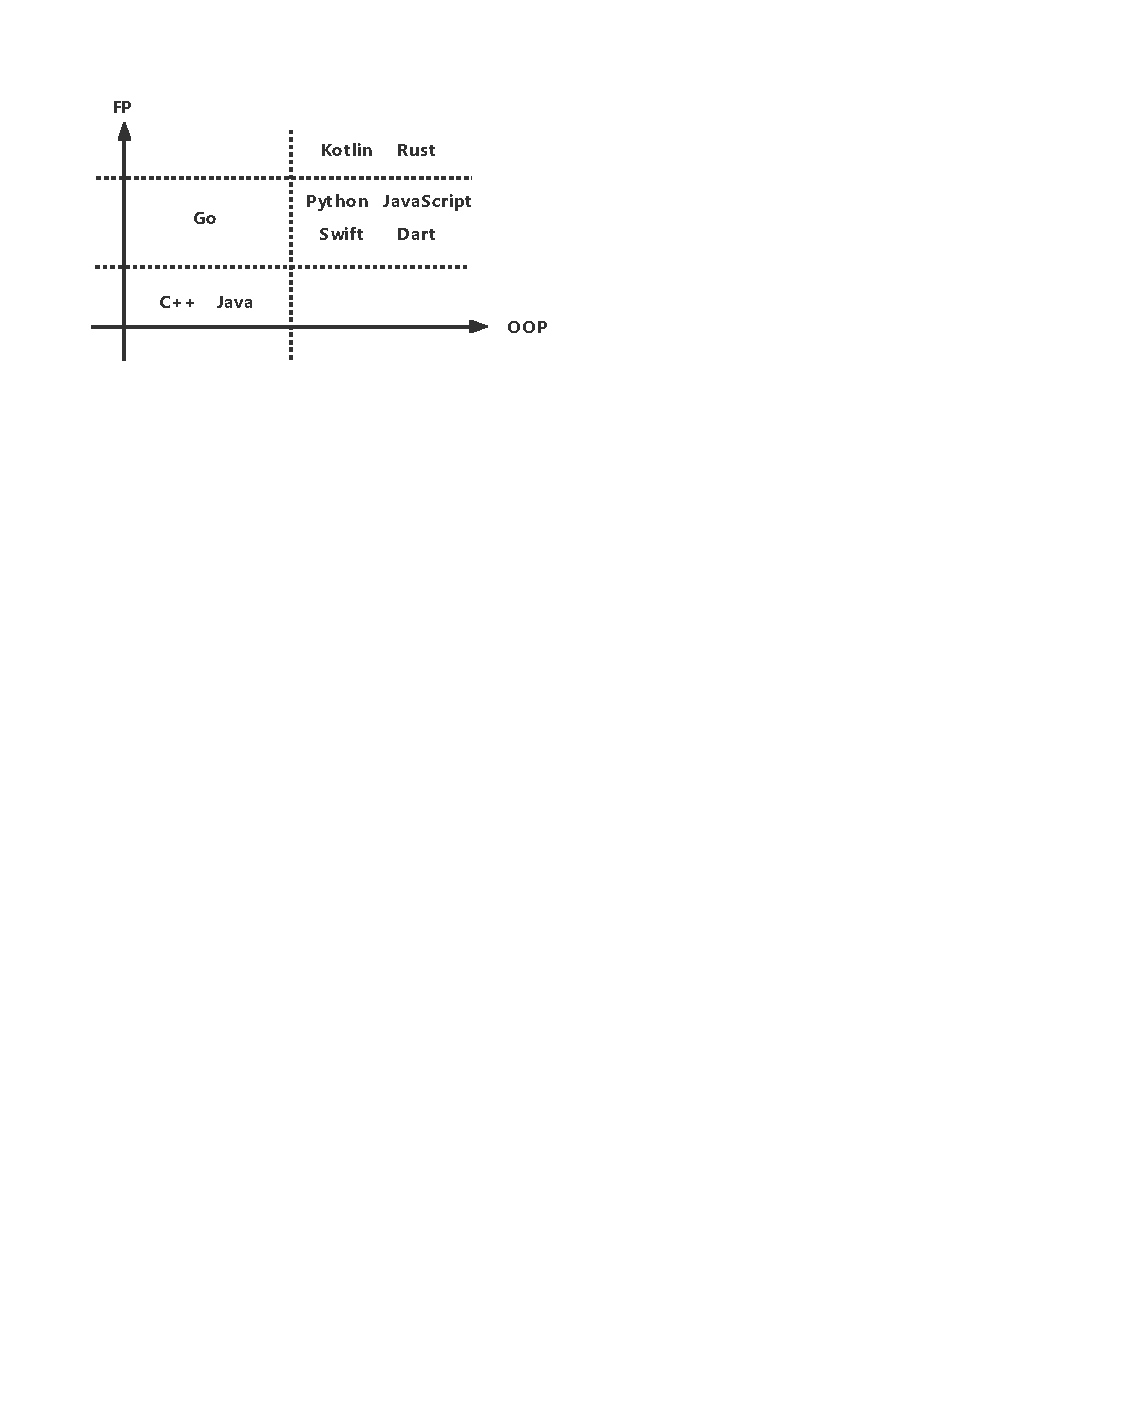
\includegraphics[scale=0.8]{figures/paradigm}}
    \caption{paradigm}
    \label{fig:paradigm}
\end{figure}

The above discussion leads to a diagram that roughly depicts the degree of support for functional and object-oriented programming concepts in different programming languages. For a given programming language, the closer it is to FP/OOP in the graph, the better it supports FP/OOP. In fact, the paradigm of a programming language is very closely related to its application scenario, whether it is for a single application area or for multiple application areas.

A typical example is Dart, whose main application scenario is the web front-end, often as a support language for the GUI framework Flutter. It is obvious that most of the GUI frameworks we use have a complex inheritance structure. This is because, for GUIs, most application scenarios satisfy the Richter substitution principle, i.e., the child type can completely replace the husband type. This is a sufficient condition for using inheritance. Therefore, Dart simply provides an object-oriented concept based on inheritance.

Another example is Java, which has weaker support for both FP and OOP concepts.Java was used for Enterprise development in the early years and provided an object-oriented paradigm in order to improve code reusability. Later it was used for Web servers, which had high requirements for abstraction of business logic, so the concept of functionalism was added additionally. But because of the historical legacy, the level of support is not good.

Another example is Kotlin, which has better support for both FP and OOP. Its initial application scenario was Android. To solve the traditional Java development Android code redundancy problem, Kotlin was designed to add a lot of functional and object-oriented concepts for the Android application scenario. These beneficial features allow Kotlin to be used in other scenarios, such as server front-ends and back-ends.


    \section{Type system}

\begin{figure}[htbp]
    \centerline{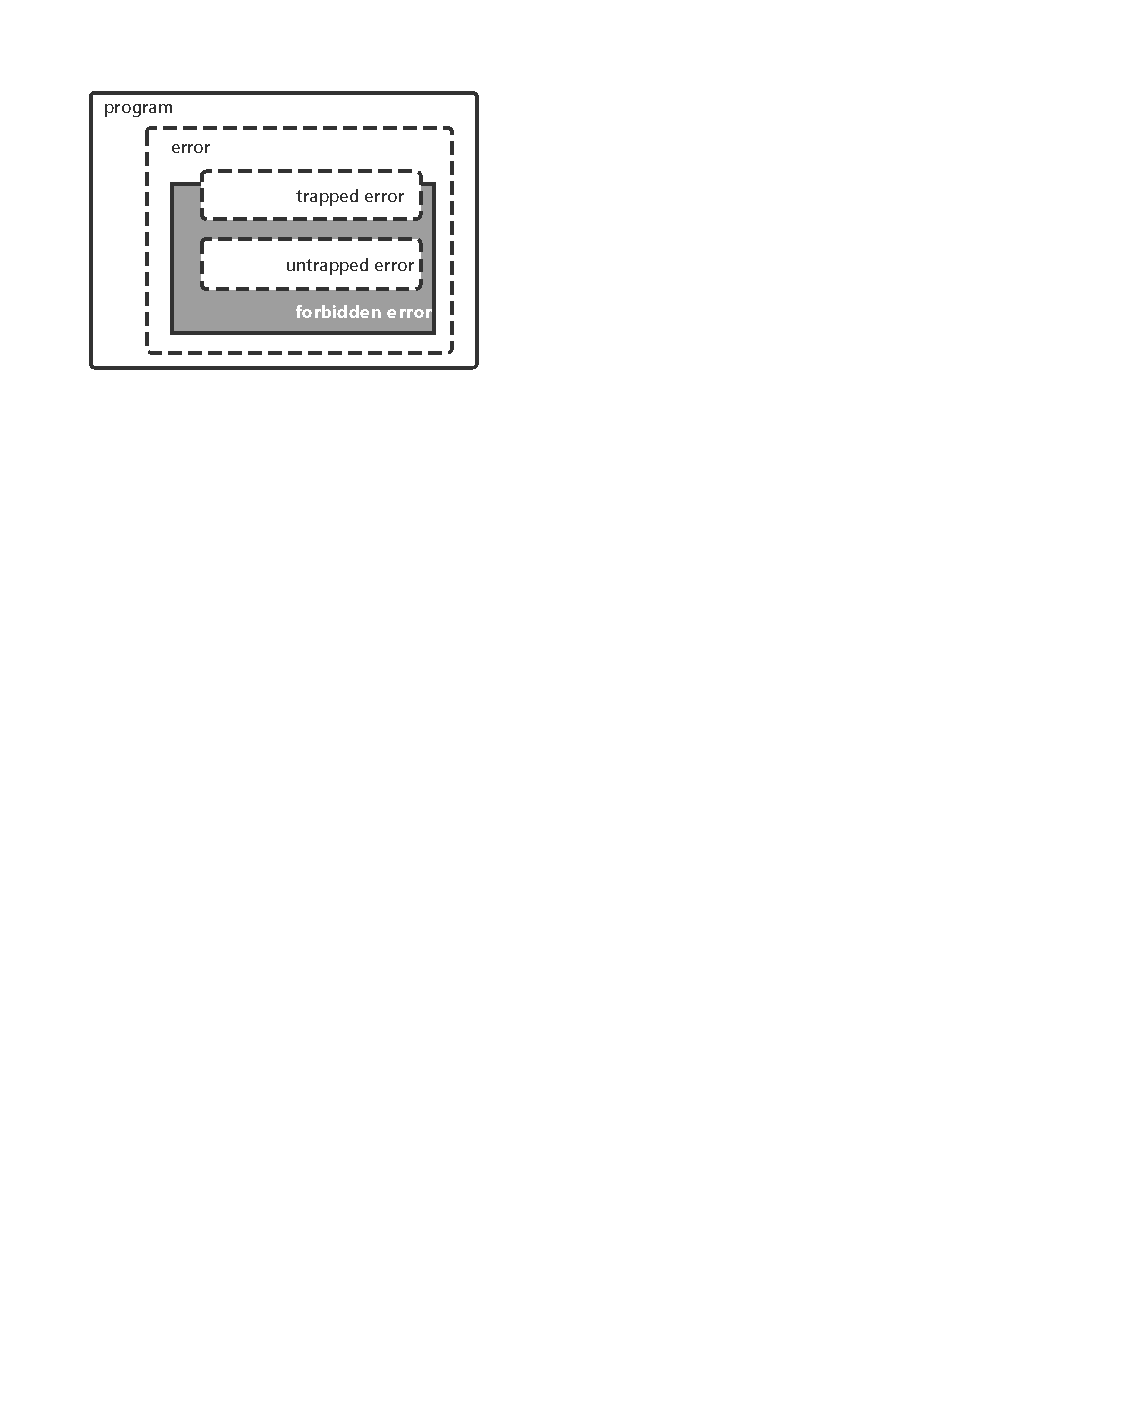
\includegraphics[scale=0.8]{figures/type-definition}}
    \caption{type-definition}
    \label{fig:type-definition}
\end{figure}


For definitional precision, the type system definition of L Cardelli is adopted here. This definition assumes that the fundamental purpose of the type system is to prevent errors that occur during the operation of a program, and therefore defines the type system by defining the concepts associated with errors. First defining what an error is to define good behavior. Then, according to the timing of behavior checking, it is divided into dynamic checking and static checking. On the basis of static checking, strong type checking and weak type checking are divided by whether forbidden error can be checked or not. As for the actual types in programming languages, they are divided into typed (static) languages and untyped (static) languages based on whether or not static types exist to limit the scope of runtime variables. Explicitly typed languages and implicitly typed languages are further divided according to whether the type of the variable is explicitly specified or not.

A very confusing issue is that the definition of the type system of programming languages varies from context to context. And there is a part of the population that discusses the types of programming languages without specifying the definition of the type system, which can easily lead to meaningless arguments about the type system in practice. A part of the population believes that JavaScript is a dynamic, weakly typed language, not an untyped language as judged here. This way of judging is also correct. In fact, the definition of this judgment criterion is based on values and variables, not on error checking as here. Another thing worth discussing is Python. type hints were introduced in Python in version 3.5. but in fact type hints do not actually error check Python, but are merely a type annotation to help provide better support for static analysis syntax parsers. The real time for error checking is still at runtime.


\begin{table*}[ht]
    \caption{type}
    \label{tab:type}
    \begin{center}
        \begin{tabular}{cccccc}
            \toprule
            Language & Typed/Untyped & Explicitly/Implicitly typed &
            Dynamically/Statically checked & Strongly/Weakly checked & Well behaved\\
            \midrule
            Python     & Typed   & Implicitly & Dynamically & Strongly & Yes \\
            Java       & Typed   & Explicitly & Statically  & Strongly & Yes \\
            C++        & Typed   & Explicitly & Statically  & Weakly   & No  \\
            JavaScript & Untyped & -          & Dynamically & -        & Yes \\
            Go         & Typed   & Explicitly & Statically  & Strongly & Yes \\
            Swift      & Typed   & Explicitly & Statically  & Strongly & Yes \\
            Dart       & Typed   & Explicitly & Statically  & Strongly & Yes \\
            Rust       & Typed   & Explicitly & Statically  & Strongly & Yes \\
            Kotlin     & Typed   & Explicitly & Statically  & Strongly & Yes \\
            \bottomrule
        \end{tabular}
    \end{center}
\end{table*}

The role of the type system for programming languages is obvious.

\begin{enumerate}
    \item Reduced expressiveness. Compared to untyped languages, the expressiveness of typed languages is somewhat reduced. But expressiveness can be improved by increasing the complexity of the type system, such as paradigms, union types, etc.
    \item Improved maintainability. Type signatures contain constraint information, and the function of a variable or function can be indirectly determined by the type signature.
    \item Improved reliability. First, the type system provides a means to check for errors. Second, the correctness of a program can be proved formally by the type system.
    \item Improved performance. First, untyped languages incur additional performance overhead at runtime for type checking and conversion. Second, typelessness is not conducive to compilation optimization. Some common JIT optimizations such as loop expansion are difficult to perform in untyped languages. Third, untyped memory memory allocation is more inefficient.
\end{enumerate}


    \section{Programming Language Performance}


There is often a debate in industry about the efficiency of programming languages, as the execution efficiency of a program often represents the performance of the program. For the same hardware conditions, a programming language that executes more efficiently often means greater load, lower latency, which is reflected in the real world as a better user experience and lower cost. The debate about programming language performance has been going on since the dawn of computing, but when it comes to performance today, most people tend to agree that C++ has higher performance than Java, and that C++ should be used to write high-performance computing because of its high performance. This is not wrong, but most people don't understand what they are talking about when they talk about the performance of programming languages. There are many factors that affect the performance of a programming language, and one cannot simply assume that one language has higher performance than another, especially if there is a specific application scenario, and the performance of a programming language is often closely related to the setting of the scenario. This leads to the concept of benchmarking.

Benchmarking provides a way to systematically test the performance differences of different individuals under the same category, providing a basis for scientifically judging individual merits. Generally in computer science, benchmarking refers to the evaluation of the performance of an object by running a particular computer program or a particular behavior of some operation, usually through a series of comparative experiments with controlled variables usually involving several iterative rounds in order to draw reproducible and precise conclusions. In addition, it focuses on a particular program and should exclude the influence of unrelated programs on the benchmark test, which requires that the benchmark test should have a clear idea of the underlying workings and avoid errors due to state uncertainty of the system. Benchmarking was first applied to computer hardware in computing, a common example being the floating-point performance of GPUs. But in recent years it can also be used for computer software, for example benchmarking compilers and databases.

\subsection{Factors affecting the performance of programming languages}

In terms of impact coverage alone, compilation principles have the greatest impact on the efficiency of programming languages. In industrial applications, the performance bottleneck in most scenarios is compile-related, where compile refers to compile in a broad sense, including not only compile-time but also run-time. The impact of compilation on programming language efficiency is again multifaceted. First, for the same programming language, using different compilers often results in different target codes and thus different runtime efficiencies, often because of different compile-time optimizations. For example, for C++, the Clang-LLVM compilation method has a significant performance difference at runtime compared to the target code obtained by using the GCC compilation method. Second, for the same programming language, it can be compiled not only in AOT (Ahead Of Time) way, but also in JIT (Just In Time) way. For example, for Kotlin, it can be compiled not only as bytecode to run on JVM, but also as JavaScript code to run on the browser, or even in Kotlin Native, compiled into native code. In this way, the different compilation methods have a greater impact on efficiency.


\begin{figure}[htbp]
    \centerline{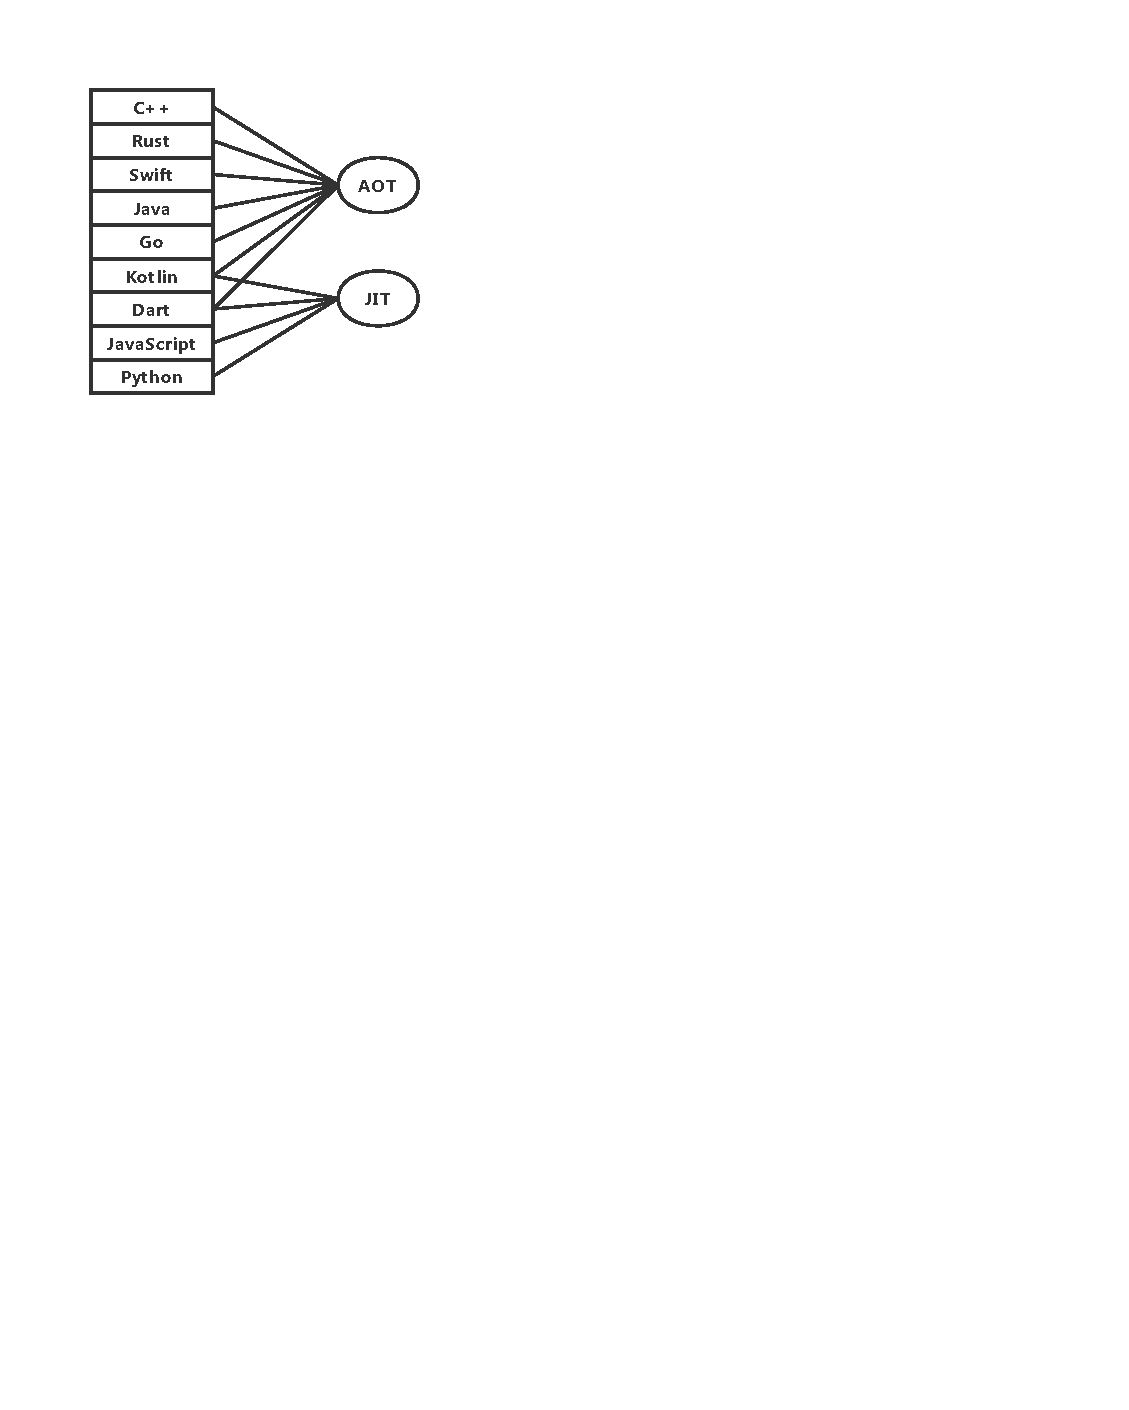
\includegraphics[scale=0.8]{figures/compilation}}
    \caption{compilation}
    \label{fig:compilation}
\end{figure}

Memory management, although not obvious in everyday use, actually has a huge impact on programming language performance. First, there is the matter of memory allocation on the heap. For languages with virtual machines, memory memory is a big advantage compared to non-VM languages. This is because VM languages tend to provide memory pools that host memory allocation, whereas non-VM languages do not have such an advantage. Of course, for scenarios where on-heap memory is used frequently, non-VM languages tend to use custom or third-party provided memory pooling frameworks, and the performance gap in industry is not as pronounced. Similarly, for VM languages, managed memory pools are not all good, and when memory jitter occurs, VMs perform frequent GCs, which also affects performance. Second, there is the principle of locality about memory. If the memory is accessed sequentially, the CPU will put all the adjacent data into the Cache, which greatly improves the hit rate of the Cache and thus the performance. Also with the compiler's loop unfolding optimization, higher efficiency is achieved. If the memory is accessed randomly, the performance is greatly reduced.

\begin{figure}[htbp]
    \centerline{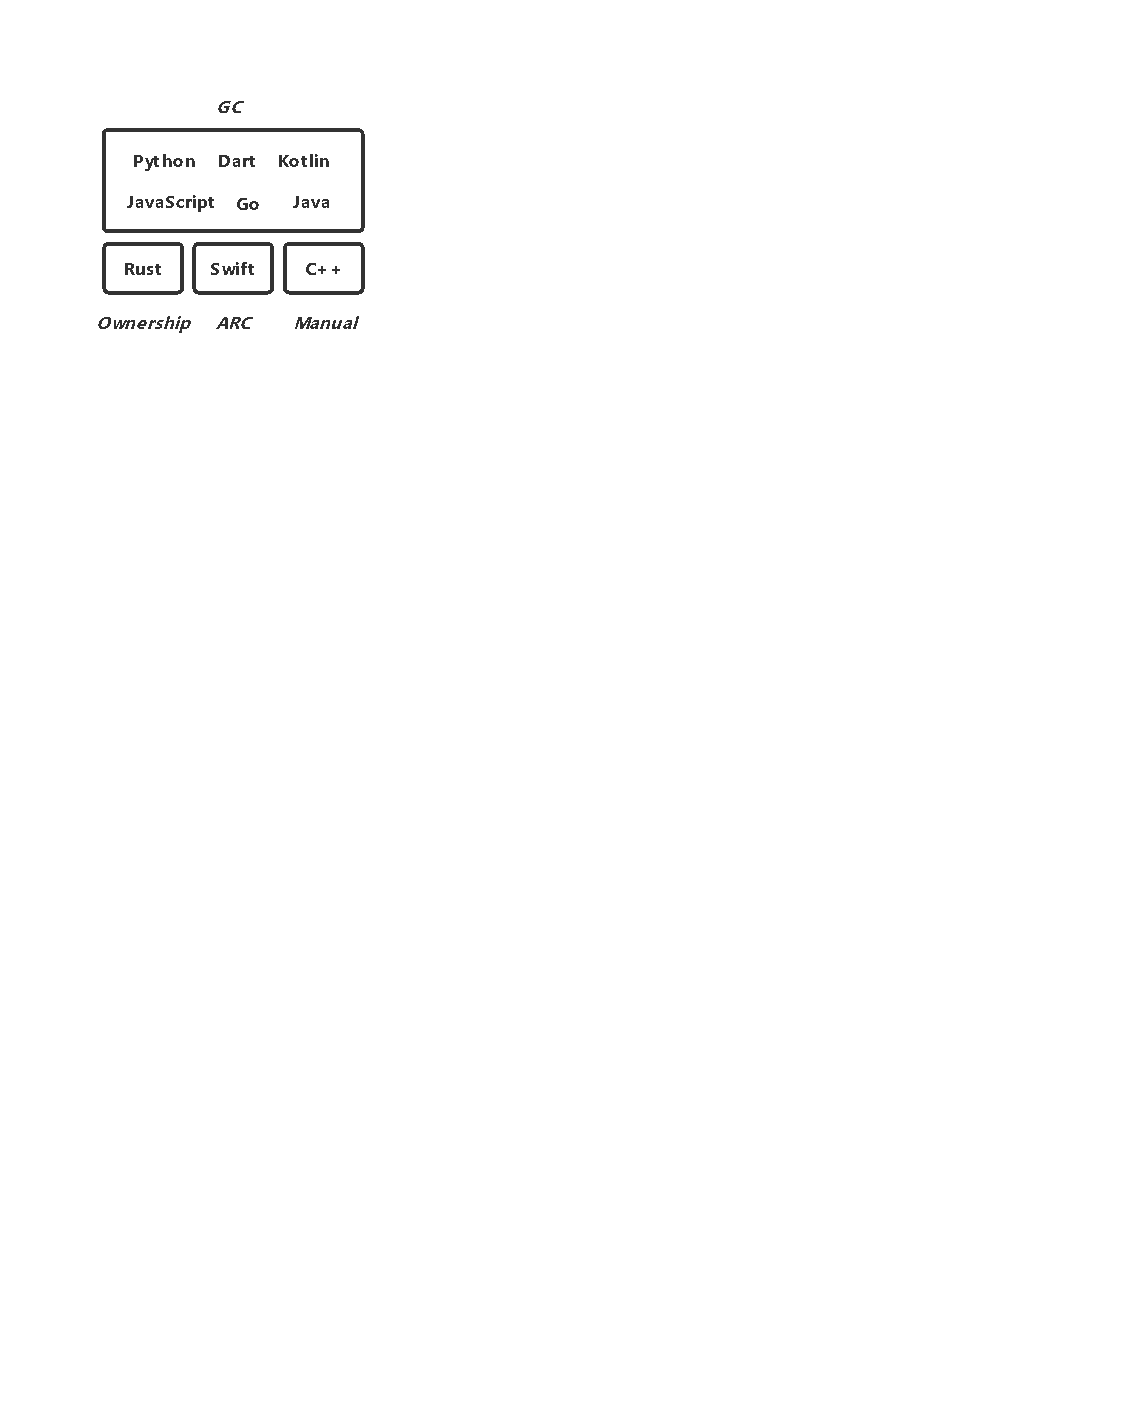
\includegraphics[scale=0.8]{figures/memory}}
    \caption{memory}
    \label{fig:memory}
\end{figure}

\subsection{Benchmarking Setup}

The dynamic metrics of the Computer Language Benchmarking Game are derived from the ideas of one of the more popular cross-language benchmarking suites available today, the Computer Language Benchmarking Game. The Computer Language Benchmarking Game currently consists of 10 benchmarking programs. Each of them provides a completely different problem for which different language specifications, language features and methods are used in an attempt to solve them using the most general way.

In this test, coarse-grained batch testing is performed uniformly using Python scripts, using built-in process tools to invoke Linux system commands, without relying on third-party libraries. It has high testing efficiency and is suitable for testing large amounts of data. Execution is performed six times for each test program and averaged to avoid errors. Each benchmark test was executed with larger and smaller scale inputs. The parameters of the testbed used, see table. The compilation parameters of the programming language, see Table.

Come for the same language with different compilers or compilation methods, the differences brought by the different compilation methods are compared (e.g. C++, Dart). The remaining languages are classified according to the programming language type system and execution method. Because for multiple languages with the same type system and compilation method, there should be an overlap in their scope of application in practice, the comparative analysis.


\begin{table}[ht]
    \caption{version}
    \label{tab:version}
    \begin{center}
        \begin{tabular}{ccc}
            \toprule
            Language   & Version         & Dependency \\
            \midrule
            Python     & CPython3.8      &            \\
            Java       & OpenJDK17       &            \\
            C++        & Clang14/GCC11.2 &            \\
            JavaScript & Node16          &            \\
            Go         & Go1.17          &            \\
            Swift      & Swift5.5        &            \\
            Dart       & Dart2.16        &            \\
            Rust       & Rust1.54        & MinGW7.3   \\
            Kotlin     & Kotlin1.6       & OpenJDK8   \\
            \bottomrule
        \end{tabular}
    \end{center}
\end{table}


For each language, there are 4 test metrics, which are:

\begin{enumerate}
    \item Compiler. Marked after the programming language, if not marked then the official compiler is used.
    \item gzip. gzip is a transfer compression protocol commonly used in industry. It is used to represent the size of the source code after compression. For the same algorithm, the smaller the amount of code used in a given programming language, the more syntactically expressive the language can be considered, in general.
    \item Time. The amount of time required to run the algorithm. Expressed as the minimum value of multiple runs. Includes startup time.
    \item Memory. The peak space consumption to run the algorithm. Expressed as the maximum of multiple runs.
\end{enumerate}

\subsection{binary-trees}

The idea is derived from Hans-J. Boehm's GC bench algorithm. The memory allocation capacity and garbage collection capacity are measured by repeatedly allocating and reclaiming space in large quantities. The steps are as follows.

\begin{figure}[htbp]
    \centerline{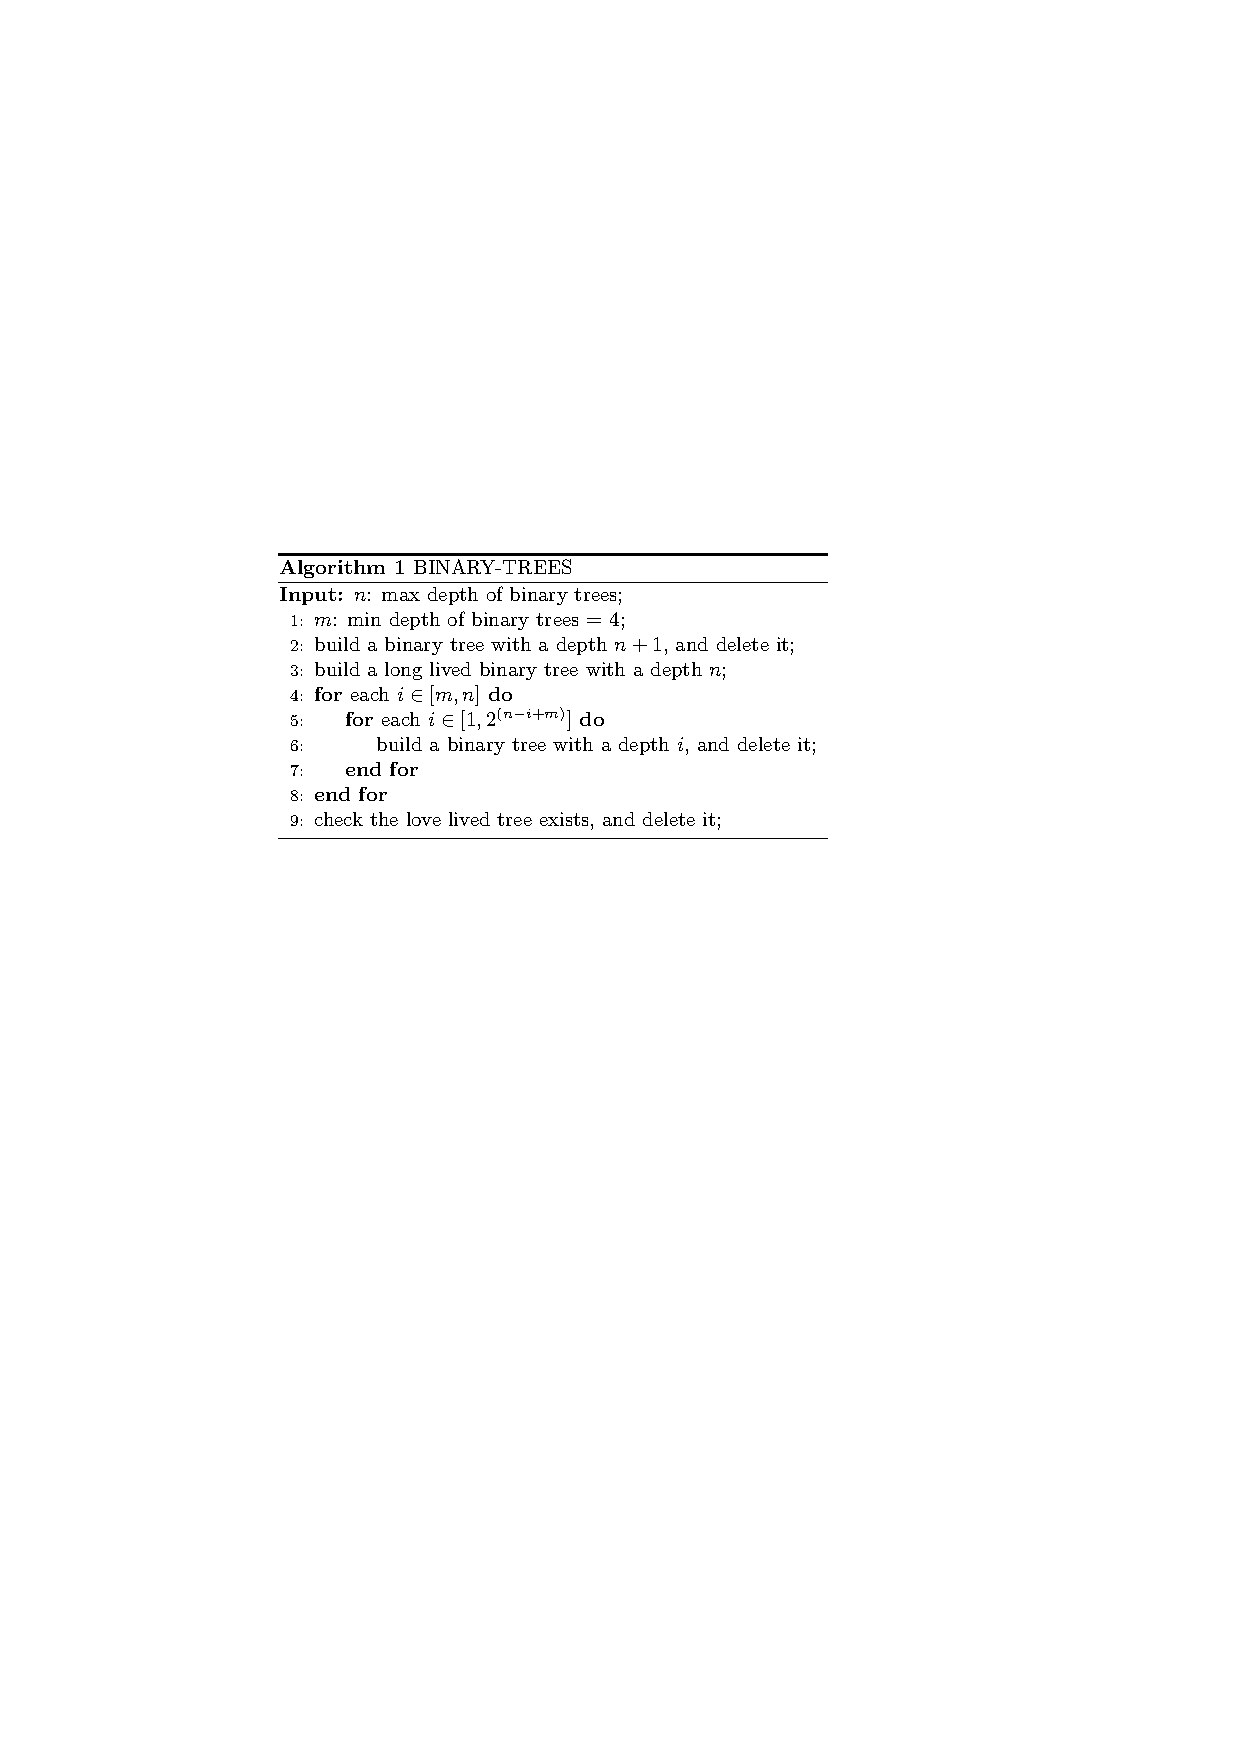
\includegraphics[scale=0.8]{figures/binary-trees}}
    \caption{binary-trees}
    \label{fig:binary-trees}
\end{figure}


\begin{table}[ht]
    \caption{binary-trees-1}
    \label{tab:binary-trees-1}
    \begin{center}
        \begin{tabular}{lrrrr}
            \toprule
            {}        & n  & size(B) & cpu(s)  & mem(KB) \\
            lang      &    &         &         &         \\
            \midrule
            cpp-clang & 21 & 654     & 16.438  & 263580  \\
            cpp-gcc   & 21 & 654     & 22.181  & 263620  \\
            dart-aot  & 21 & 1212    & 45.461  & 799012  \\
            dart-jit  & 21 & 1212    & 61.531  & 1626352 \\
            go        & 21 & 482     & 50.955  & 220548  \\
            java      & 21 & 552     & 5.607   & 2015512 \\
            js-node   & 21 & 711     & 36.391  & 1130788 \\
            kt-jvm    & 21 & 494     & 8.923   & 1783144 \\
            python3   & 21 & 589     & 169.912 & 442180  \\
            rust      & 21 & 751     & 7.796   & 132508  \\
            swift     & 21 & 714     & 63.608  & 733144  \\
            \bottomrule
        \end{tabular}
    \end{center}
\end{table}

\begin{table}[ht]
    \caption{binary-trees-2}
    \label{tab:binary-trees-2}
    \begin{center}
        \begin{tabular}{lrrrr}
            \toprule
            {}        & n  & size(B) & cpu(s) & mem(KB) \\
            lang      &    &         &        &         \\
            \midrule
            cpp-clang & 14 & 654     & 0.087  & 1200    \\
            cpp-gcc   & 14 & 654     & 0.104  & 3928    \\
            dart-aot  & 14 & 1212    & 0.120  & 1680    \\
            dart-jit  & 14 & 1212    & 0.644  & 170008  \\
            go        & 14 & 482     & 0.214  & 7232    \\
            java      & 14 & 552     & 0.155  & 47968   \\
            js-node   & 14 & 711     & 0.717  & 90512   \\
            kt-jvm    & 14 & 494     & 0.249  & 36040   \\
            python3   & 14 & 589     & 0.911  & 14420   \\
            rust      & 14 & 751     & 0.042  & 1176    \\
            swift     & 14 & 714     & 0.299  & 17616   \\
            \bottomrule
        \end{tabular}
    \end{center}
\end{table}

As you can see from the table, Java has the best memory allocation and management speed among these programming languages, and it takes very little time. However, Java's memory consumption is relatively the largest among these languages. This is due to the unique memory model of the JVM, which divides the heap area into different generations and uses different garbage collection algorithms for each generation. The advantage of this is obvious, it can greatly reduce the efficiency of garbage collection. But at the same time, it takes up more memory than is actually needed for the division. Since Kotlin and Java are both based on the JVM, they have similar performance figures. Kotlin is based on Java8, while Java is based on Java17. From Java9 onwards, the default JVM GC is G1. Parallel has a better response time than Parallel, but also consumes more memory. This is in perfect agreement with the data in the table that Kotlin has a slightly higher time overhead than Java and a slightly lower memory overhead than Java.

For the two different compilers for C++, Clang and GCC, the memory overheads are almost identical. This is because both of them manage memory manually. Clang, however, has a lower time consumption than GCC. This comes from the compiler optimizations, which are better in Clang than in GCC. The compiler architecture of Clang-LLVM is different. Clang-LLVM uses a low-coupling front- and back-end architecture, while GCC uses a front- and back-end coupling architecture, due to the fact that GCC is relatively old and limited by its age. This shows that compile-time optimization of the compiler is more important for a native compiled language.

Rust, Go, and Swift, which are also modern strongly typed, compiled languages, use three different memory management models. Go uses a garbage collection mechanism. Although Go is a compiled language, it has an additional runtime to support garbage collection. Compared to Java, Go uses a more conservative garbage collection strategy and does not adopt a drastic space-for-time strategy, resulting in a decent space consumption and a less optimistic runtime for memory allocation. Rust, on the other hand, uses an ownership mechanism that differs from the purely manually managed C/C++ and from Go's garbage collection. In terms of the underlying implementation, Rust does not actually maintain a runtime to manage space, but rather determines the timing of reclaiming memory at compile time through a complex arithmetic ownership algorithm. As a result, Rust's memory management is overhead-free. In fact, Rust's compiler backend uses LLVM, the same backend as the Clang-LLVM group tested above, and it is also clear from the test data that Rust performs almost identically to Cpp-Clang on floating-point operations. However, due to its ownership mechanism, Rust is better in memory allocation. For Swift, the memory management mechanism is different from all of the above. swift allocates and reclaims memory by maintaining a runtime reference count. In addition, Swift forces reference counts to be updated atomically instead of Rust's compiler management of thread safety, which results in high CPU overhead. This shows that Swift has a higher runtime overhead compared to Rust, confirming the data that Swift performs poorly compared to Rust.

\subsection{n-body}

The idea comes from the Symplectic Integration algorithm of K. P. Rauch and D. P. Hamilton simulates the evolution of multiple planets and confirms the correctness of the algorithm by checking the energy of each evolutionary state.

The performance bottleneck is mainly focused on floating-point operations. The steps are as follows.

\begin{figure}[htbp]
    \centerline{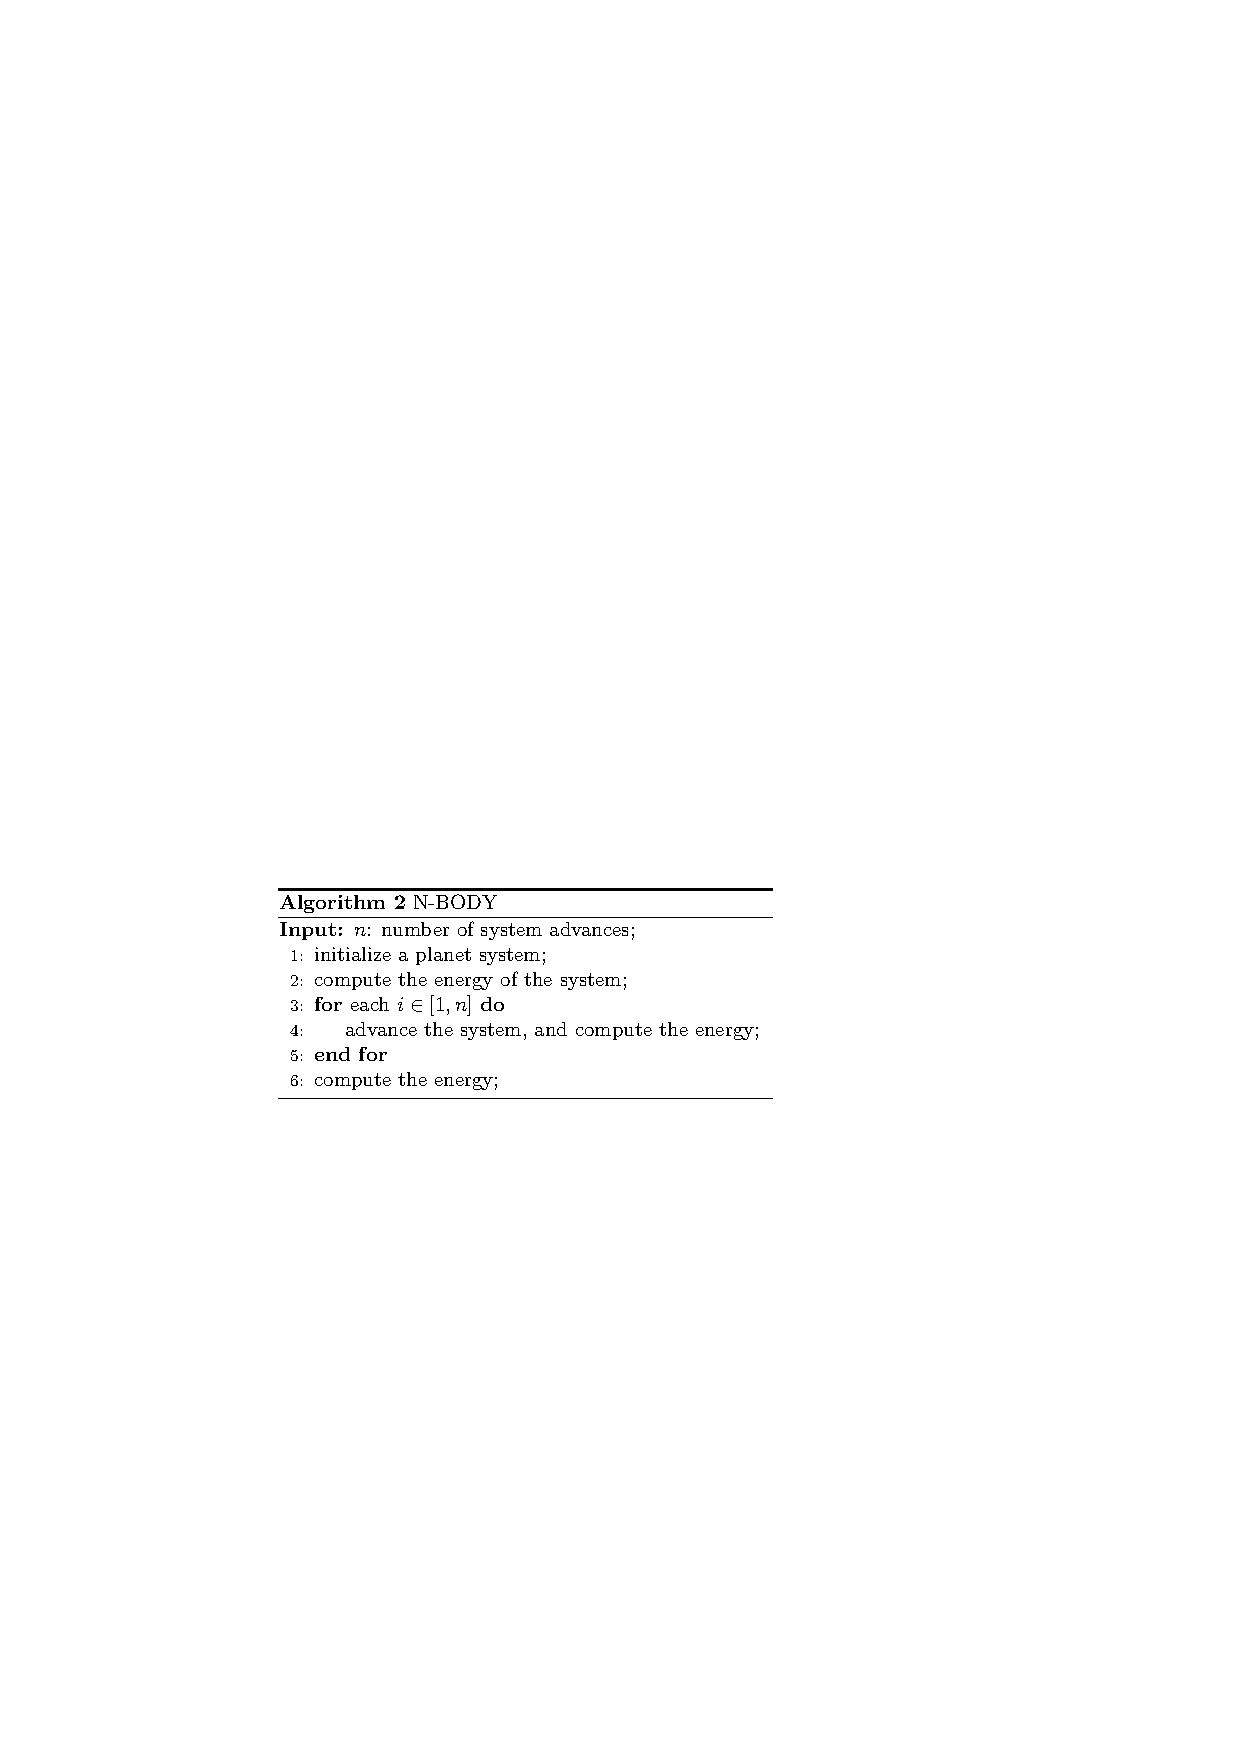
\includegraphics[scale=0.8]{figures/n-body}}
    \caption{n-body}
    \label{fig:n-body}
\end{figure}

\begin{table}[ht]
    \caption{n-body-1}
    \label{tab:n-body-1}
    \begin{center}
        \begin{tabular}{lrrrr}
            \toprule
            {}        & n        & size(B) & cpu(s)  & mem(KB) \\
            lang      &          &         &         &         \\
            \midrule
            cpp-clang & 50000000 & 1173    & 5.926   & 1236    \\
            cpp-gcc   & 50000000 & 1173    & 7.555   & 1228    \\
            dart-aot  & 50000000 & 1266    & 10.220  & 9308    \\
            dart-jit  & 50000000 & 1266    & 13.193  & 143436  \\
            go        & 50000000 & 1310    & 6.581   & 1128    \\
            java      & 50000000 & 1430    & 7.816   & 37260   \\
            js-node   & 50000000 & 1268    & 8.550   & 39956   \\
            kt-jvm    & 50000000 & 1124    & 6.914   & 37068   \\
            python3   & 50000000 & 1196    & 541.319 & 7780    \\
            rust      & 50000000 & 1480    & 5.818   & 1024    \\
            swift     & 50000000 & 1192    & 9.585   & 6308    \\
            \bottomrule
        \end{tabular}
    \end{center}
\end{table}


\begin{table}[ht]
    \caption{n-body-2}
    \label{tab:n-body-2}
    \begin{center}
        \begin{tabular}{lrrrr}
            \toprule
            {}        & n       & size(B) & cpu(s) & mem(KB) \\
            lang      &         &         &        &         \\
            \midrule
            cpp-clang & 5000000 & 1173    & 0.621  & 1204    \\
            cpp-gcc   & 5000000 & 1173    & 0.766  & 1204    \\
            dart-aot  & 5000000 & 1266    & 1.033  & 9216    \\
            dart-jit  & 5000000 & 1266    & 1.918  & 143256  \\
            go        & 5000000 & 1310    & 0.661  & 816     \\
            java      & 5000000 & 1430    & 0.880  & 37460   \\
            js-node   & 5000000 & 1268    & 0.941  & 39864   \\
            kt-jvm    & 5000000 & 1124    & 0.826  & 37064   \\
            python3   & 5000000 & 1196    & 52.530 & 7800    \\
            rust      & 5000000 & 1480    & 0.579  & 1020    \\
            swift     & 5000000 & 1192    & 0.976  & 6308    \\
            \bottomrule
        \end{tabular}
    \end{center}
\end{table}


Java's time consumption is not very high and does not fall too far behind native compiled languages. The performance bottleneck of algorithmic programs with short total runtime in Java is mainly the JVM startup time and the JIT-optimized warm-up time, and for algorithms that are already warmed up, Java's execution speed does not lag behind that of native compiled languages. Java runs in two steps. In the first step, the source code is compiled into bytecode, and in the second step, the JVM interprets and executes the bytecode. In the process of interpreting and executing the bytecode, JVM will receive the runtime information of the set code, and if it finds that some bytecode is executed more frequently, it will choose to compile this part of bytecode into native code, and call the native code directly when it is executed again. The so-called performance optimization of Java is mainly focused on the compilation stage of bytecode, while the source-to-bytecode stage is only simply optimized.

There is a significant performance gap between JavaScript and Python, and JavaScript has excellent performance with Google's V8 engine, which executes js code much like the Java virtual machine executes bytecode, using the same JIT optimization technology, so compared to Python, which does not use JIT optimization, it So compared to Python, which does not use JIT optimization, it has a huge performance improvement, and even has a similar floating-point performance to Java and native compiled languages. In fact, the speed of scripting languages is not a performance bottleneck in most application scenarios. However, in recent years, JavaScript has become the "assembly of the web", and more and more languages are being compiled into JavaScript, such as Kotlin, Dart, etc. As a result, more and more business logic needs to be executed in JavaScript, which makes This makes JavaScript burdened with tedious business-related logic, and the trend is to optimize JavaScript.

\subsection{mandelbrot}

\begin{figure}[htbp]
    \centerline{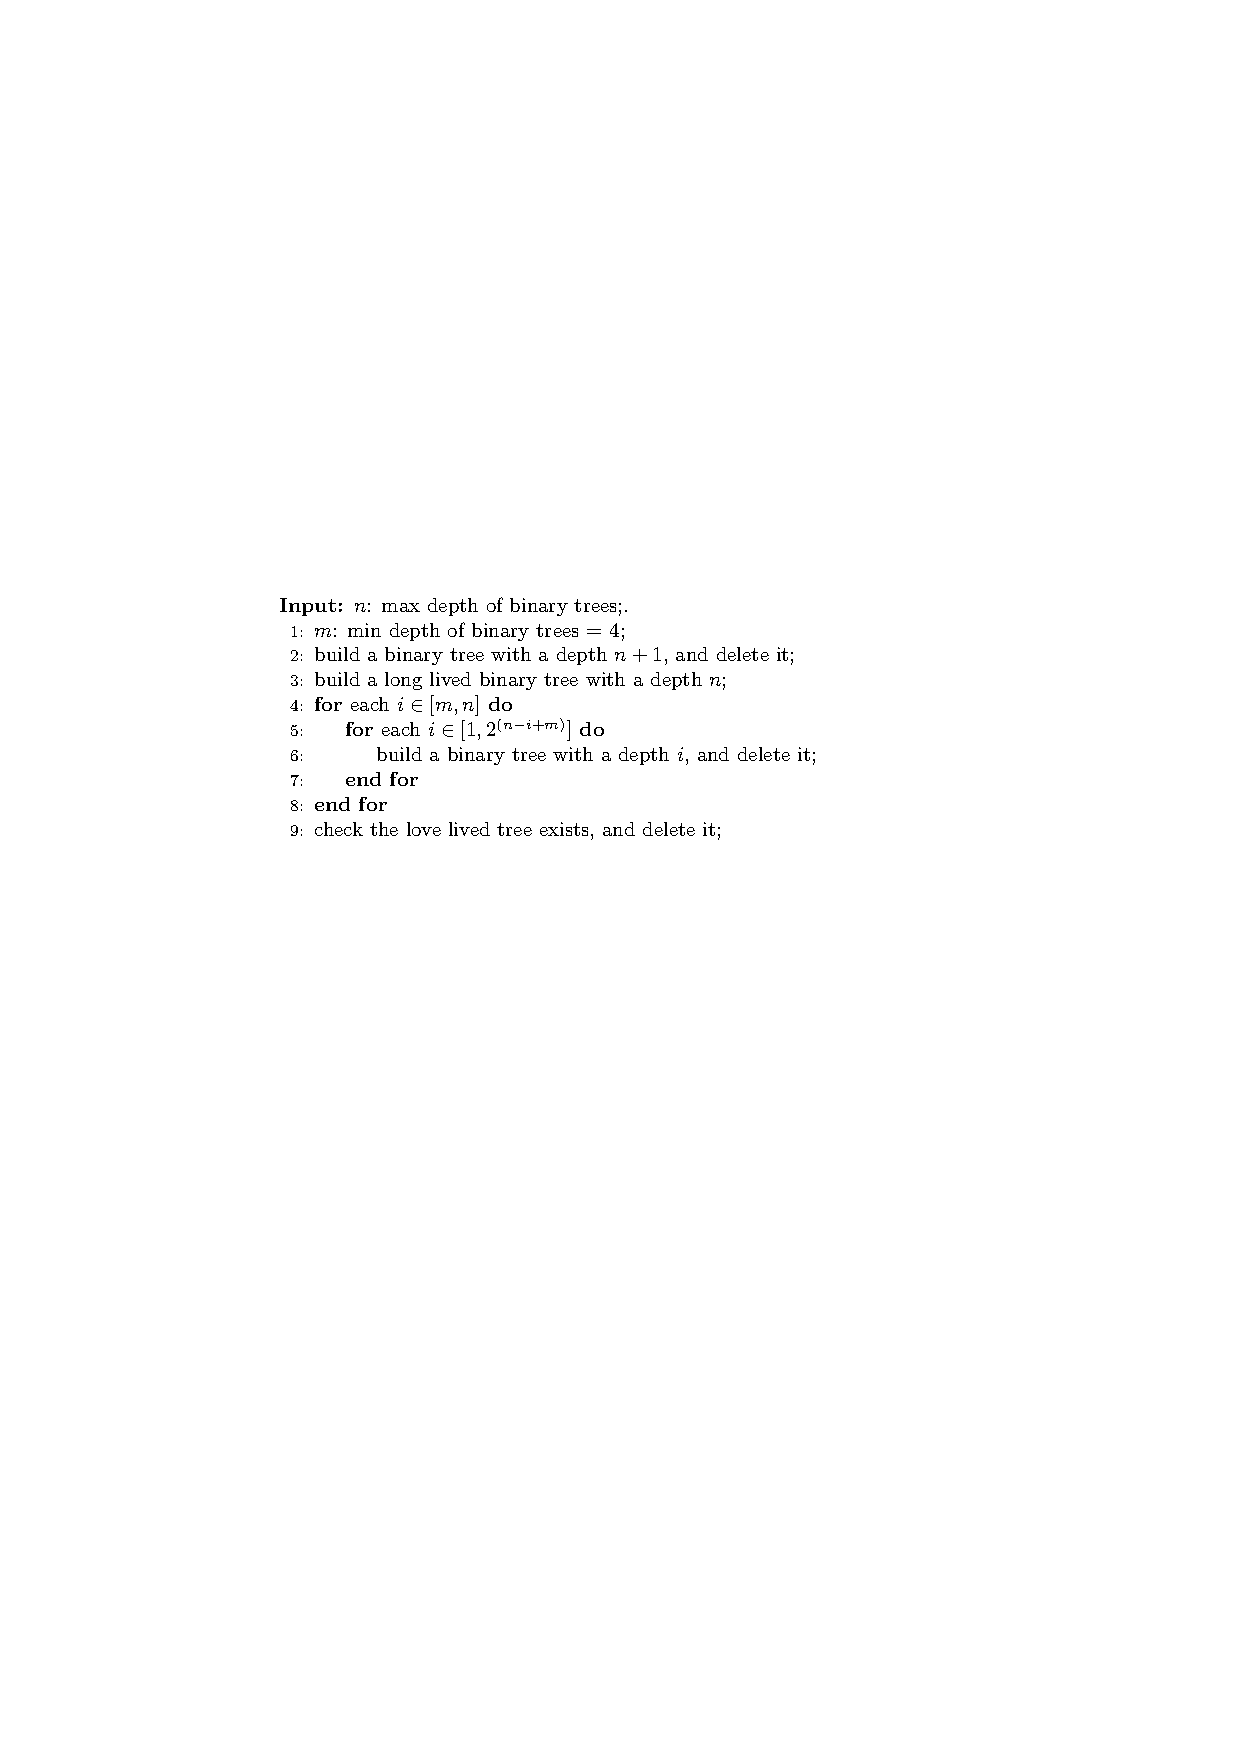
\includegraphics[scale=0.8]{figures/mandelbrot}}
    \caption{mandelbrot}
    \label{fig:mandelbrot}
\end{figure}

\begin{table}[ht]
    \caption{mandelbrot-1}
    \label{tab:mandelbrot-1}
    \begin{center}
        \begin{tabular}{lrrrr}
            \toprule
            {}        & n     & size(B) & cpu(s)  & mem(KB) \\
            lang      &       &         &         &         \\
            \midrule
            cpp-clang & 16000 & 822     & 13.900  & 30172   \\
            cpp-gcc   & 16000 & 822     & 13.931  & 28696   \\
            dart-aot  & 16000 & 454     & 154.089 & 17240   \\
            dart-jit  & 16000 & 454     & 151.501 & 148144  \\
            go        & 16000 & 823     & 19.598  & 32412   \\
            java      & 16000 & 665     & 27.834  & 34264   \\
            js-node   & 16000 & 373     & 130.638 & 42020   \\
            kt-jvm    & 16000 & 407     & 30.032  & 28432   \\
            python3   & 16000 & 688     & 702.599 & 47780   \\
            rust      & 16000 & 868     & 11.904  & 38528   \\
            swift     & 16000 & 394     & 26.277  & 6200    \\
            \bottomrule
        \end{tabular}
    \end{center}
\end{table}


\begin{table}[ht]
    \caption{mandelbrot-2}
    \label{tab:mandelbrot-2}
    \begin{center}
        \begin{tabular}{lrrrr}
            \toprule
            {}        & n    & size(B) & cpu(s) & mem(KB) \\
            lang      &      &         &        &         \\
            \midrule
            cpp-clang & 4000 & 822     & 0.880  & 1552    \\
            cpp-gcc   & 4000 & 822     & 0.881  & 1192    \\
            dart-aot  & 4000 & 454     & 10.276 & 17380   \\
            dart-jit  & 4000 & 454     & 10.096 & 148084  \\
            go        & 4000 & 823     & 1.260  & 2420    \\
            java      & 4000 & 665     & 1.827  & 34352   \\
            js-node   & 4000 & 373     & 8.763  & 42540   \\
            kt-jvm    & 4000 & 407     & 2.419  & 28448   \\
            python3   & 4000 & 688     & 46.273 & 12172   \\
            rust      & 4000 & 868     & 0.757  & 4388    \\
            swift     & 4000 & 394     & 1.661  & 6240    \\
            \bottomrule
        \end{tabular}
    \end{center}
\end{table}

For the same Dart code, two different ways of compiling are used, JIT and AOT. For memory overhead, AOT has a definite advantage over JIT for both. While for time overhead, both have similar performance. This is caused by the compilation mechanism of Dart. In fact, the compilation and running mechanism of Dart is different from both the traditional way. The traditional AOT is to compile the program code directly into the target code on the target machine, which can be called and run independently by the operating system directly. However, for Dart, whether it is AOT or JIT, only the compilation time is different, and it will eventually be run on the virtual machine. In fact, when the compilation time is negligible, the time overhead of AOT and JIT is approximately equal. But this way of running has its unique disadvantage, it will significantly increase the running overhead of AOT mode, but this makes AOT compilation has a strong runtime support. Because of this feature, the Dart VM can save the current runtime state, and the next time the VM is started, it can directly load the last state without restarting. This is done mainly for a smooth development experience, and the incremental compilation feature allows the runtime results to change almost in real time as the code is changed, with minimal latency. This design is because Dart is mainly used as the development language for the front-end cross-platform framework Flutter, allowing real-time feedback on changes to the UI interface, which is difficult to do in other languages.



    \section{summary}

As we can see, new compilation techniques are always emerging as programming languages evolve. The analysis of modern programming languages from the perspective of language design is often limited by the times. In this paper, we start from the current development status of programming languages, and provide some reference for the development direction and application scenarios of programming languages by studying the impact of each component of programming language design on the programming language itself. Programming paradigms, type systems, and performance are three interrelated components that cut across multiple aspects of programming languages from design to implementation. Each of these three branches itself has a significant impact on the design of programming languages, influencing their expressiveness, maintainability, reliability, and performance, the most important indicators of programming languages. In fact we can obtain that the process of theoretical and practical development of programming languages is always dynamic, as is the design and implementation of programming languages. This paper dynamically talks about the design of programming languages from the perspective of modern programming languages, which would be a better research idea from the perspective of programming language design and analysis.

%    \section{Ease of Use}

\subsection{Maintaining the Integrity of the Specifications}

The IEEEtran class file is used to format your paper and style the text. All margins,
column widths, line spaces, and text fonts are prescribed; please do not
alter them. You may note peculiarities. For example, the head margin
measures proportionately more than is customary. This measurement
and others are deliberate, using specifications that anticipate your paper
as one part of the entire proceedings, and not as an independent document.
Please do not revise any of the current designations.


\section{Prepare Your Paper Before Styling}
Before you begin to format your paper, first write and save the content as a
separate text file. Complete all content and organizational editing before
formatting. Please note sections \ref{AA}--\ref{SCM} below for more information on
proofreading, spelling and grammar.

Keep your text and graphic files separate until after the text has been
formatted and styled. Do not number text heads---{\LaTeX} will do that
for you.

\subsection{Abbreviations and Acronyms}\label{AA}
Define abbreviations and acronyms the first time they are used in the text,
even after they have been defined in the abstract. Abbreviations such as
IEEE, SI, MKS, CGS, ac, dc, and rms do not have to be defined. Do not use
abbreviations in the title or heads unless they are unavoidable.

\subsection{Units}
\begin{itemize}
    \item Use either SI (MKS) or CGS as primary units. (SI units are encouraged.) English units may be used as secondary units (in parentheses). An exception would be the use of English units as identifiers in trade, such as ``3.5-inch disk drive''.
    \item Avoid combining SI and CGS units, such as current in amperes and magnetic field in oersteds. This often leads to confusion because equations do not balance dimensionally. If you must use mixed units, clearly state the units for each quantity that you use in an equation.
    \item Do not mix complete spellings and abbreviations of units: ``Wb/m\textsuperscript{2}'' or ``webers per square meter'', not ``webers/m\textsuperscript{2}''. Spell out units when they appear in text: ``. . . a few henries'', not ``. . . a few H''.
    \item Use a zero before decimal points: ``0.25'', not ``.25''. Use ``cm\textsuperscript{3}'', not ``cc''.)
\end{itemize}

\subsection{Equations}
Number equations consecutively. To make your
equations more compact, you may use the solidus (~/~), the exp function, or
appropriate exponents. Italicize Roman symbols for quantities and variables,
but not Greek symbols. Use a long dash rather than a hyphen for a minus
sign. Punctuate equations with commas or periods when they are part of a
sentence, as in:
\begin{equation}
    a+b=\gamma\label{eq}
\end{equation}

Be sure that the
symbols in your equation have been defined before or immediately following
the equation. Use ``\eqref{eq}'', not ``Eq.~\eqref{eq}'' or ``equation \eqref{eq}'', except at
the beginning of a sentence: ``Equation \eqref{eq} is . . .''

\subsection{\LaTeX-Specific Advice}

Please use ``soft'' (e.g., \verb|\eqref{Eq}|) cross references instead
of ``hard'' references (e.g., \verb|(1)|). That will make it possible
to combine sections, add equations, or change the order of figures or
citations without having to go through the file line by line.

Please don't use the \verb|{eqnarray}| equation environment. Use
\verb|{align}| or \verb|{IEEEeqnarray}| instead. The \verb|{eqnarray}|
environment leaves unsightly spaces around relation symbols.

Please note that the \verb|{subequations}| environment in {\LaTeX}
will increment the main equation counter even when there are no
equation numbers displayed. If you forget that, you might write an
article in which the equation numbers skip from (17) to (20), causing
the copy editors to wonder if you've discovered a new method of
counting.

    {\BibTeX} does not work by magic. It doesn't get the bibliographic
data from thin air but from .bib files. If you use {\BibTeX} to produce a
bibliography you must send the .bib files.

    {\LaTeX} can't read your mind. If you assign the same label to a
subsubsection and a table, you might find that Table I has been cross
referenced as Table IV-B3.

    {\LaTeX} does not have precognitive abilities. If you put a
\verb|\label| command before the command that updates the counter it's
supposed to be using, the label will pick up the last counter to be
cross referenced instead. In particular, a \verb|\label| command
should not go before the caption of a figure or a table.

Do not use \verb|\nonumber| inside the \verb|{array}| environment. It
will not stop equation numbers inside \verb|{array}| (there won't be
any anyway) and it might stop a wanted equation number in the
surrounding equation.

\subsection{Some Common Mistakes}\label{SCM}
\begin{itemize}
    \item The word ``data'' is plural, not singular.
    \item The subscript for the permeability of vacuum $\mu_{0}$, and other common scientific constants, is zero with subscript formatting, not a lowercase letter ``o''.
    \item In American English, commas, semicolons, periods, question and exclamation marks are located within quotation marks only when a complete thought or name is cited, such as a title or full quotation. When quotation marks are used, instead of a bold or italic typeface, to highlight a word or phrase, punctuation should appear outside of the quotation marks. A parenthetical phrase or statement at the end of a sentence is punctuated outside of the closing parenthesis (like this). (A parenthetical sentence is punctuated within the parentheses.)
    \item A graph within a graph is an ``inset'', not an ``insert''. The word alternatively is preferred to the word ``alternately'' (unless you really mean something that alternates).
    \item Do not use the word ``essentially'' to mean ``approximately'' or ``effectively''.
    \item In your paper title, if the words ``that uses'' can accurately replace the word ``using'', capitalize the ``u''; if not, keep using lower-cased.
    \item Be aware of the different meanings of the homophones ``affect'' and ``effect'', ``complement'' and ``compliment'', ``discreet'' and ``discrete'', ``principal'' and ``principle''.
    \item Do not confuse ``imply'' and ``infer''.
    \item The prefix ``non'' is not a word; it should be joined to the word it modifies, usually without a hyphen.
    \item There is no period after the ``et'' in the Latin abbreviation ``et al.''.
    \item The abbreviation ``i.e.'' means ``that is'', and the abbreviation ``e.g.'' means ``for example''.
\end{itemize}
An excellent style manual for science writers is \cite{b7}.

\subsection{Authors and Affiliations}
\textbf{The class file is designed for, but not limited to, six authors.} A
minimum of one author is required for all conference articles. Author names
should be listed starting from left to right and then moving down to the
next line. This is the author sequence that will be used in future citations
and by indexing services. Names should not be listed in columns nor group by
affiliation. Please keep your affiliations as succinct as possible (for
example, do not differentiate among departments of the same organization).

\subsection{Identify the Headings}
Headings, or heads, are organizational devices that guide the reader through
your paper. There are two types: component heads and text heads.

Component heads identify the different components of your paper and are not
topically subordinate to each other. Examples include Acknowledgments and
References and, for these, the correct style to use is ``Heading 5''. Use
``figure caption'' for your Figure captions, and ``table head'' for your
table title. Run-in heads, such as ``Abstract'', will require you to apply a
style (in this case, italic) in addition to the style provided by the drop
down menu to differentiate the head from the text.

Text heads organize the topics on a relational, hierarchical basis. For
example, the paper title is the primary text head because all subsequent
material relates and elaborates on this one topic. If there are two or more
sub-topics, the next level head (uppercase Roman numerals) should be used
and, conversely, if there are not at least two sub-topics, then no subheads
should be introduced.

\subsection{Figures and Tables}

\paragraph{Positioning Figures and Tables} Place figures and tables at the top and
bottom of columns. Avoid placing them in the middle of columns. Large
figures and tables may span across both columns. Figure captions should be
below the figures; table heads should appear above the tables. Insert
figures and tables after they are cited in the text. Use the abbreviation
``Fig.~\ref{fig}'', even at the beginning of a sentence.

\begin{table}[htbp]
    \caption{Table Type Styles}
    \begin{center}
        \begin{tabular}{|c|c|c|c|}
            \hline
            \textbf{Table} & \multicolumn{3}{|c|}{\textbf{Table Column Head}} \\
            \cline{2-4}
            \textbf{Head} & \textbf{\textit{Table column subhead}} & \textbf{\textit{Subhead}} & \textbf{\textit{Subhead}} \\
            \hline
            copy          & More table copy$^{\mathrm{a}}$         &                           &                           \\
            \hline
            \multicolumn{4}{l}{$^{\mathrm{a}}$Sample of a Table footnote.}
        \end{tabular}
        \label{tab1}
    \end{center}
\end{table}

\begin{figure}[htbp]
    \centerline{
\includegraphics{figures/fig1}}
    \caption{Example of a figure caption.}
    \label{fig}
\end{figure}

Figure Labels: Use 8 point Times New Roman for Figure labels. Use words
rather than symbols or abbreviations when writing Figure axis labels to
avoid confusing the reader. As an example, write the quantity
``Magnetization'', or ``Magnetization, M'', not just ``M''. If including
units in the label, present them within parentheses. Do not label axes only
with units. In the example, write ``Magnetization (A/m)'' or ``Magnetization
\{A[m(1)]\}'', not just ``A/m''. Do not label axes with a ratio of
quantities and units. For example, write ``Temperature (K)'', not
``Temperature/K''.



    \bibliographystyle{IEEEtran}
    \bibliography{IEEEabrv,main}
\end{document}
